% This is a sample document using the University of Minnesota, Morris, Computer Science
% Senior Seminar modification of the ACM sig-alternate style. Much of this content is taken
% directly from the ACM sample document illustrating the use of the sig-alternate class. Certain
% parts that we never use have been removed to simplify the example, and a few additional
% components have been added.

% See https://github.com/UMM-CSci/Senior_seminar_templates for more info and to make
% suggestions and corrections.

\documentclass{sig-alternate}
\usepackage{color}



\setlength{\marginparwidth}{2cm}
\usepackage[colorinlistoftodos]{todonotes}

\usepackage{url}

\usepackage{subcaption}

\usepackage{graphicx}

\graphicspath{ {./figures/} }

\usepackage{amsmath}

\usepackage{dblfloatfix}    % To enable figures at the bottom of page

\usepackage[
bookmarksnumbered,
hidelinks,
pdflang={en},
pdfdisplaydoctitle,
pdfauthor={Paul Friederichsen},
pdftitle={Recent Advances in Smartphone Computational Photography},
pdfkeywords={computational photography, image processing, low-light imaging, photography, super-resolution}
]{hyperref}

%\urlstyle{rm}

\boilerplate={This work is licensed under the Creative Commons 
Attribution-NonCommercial-ShareAlike 4.0 International License. 
To view a copy of this license, visit 
\href{https://creativecommons.org/licenses/by-nc-sa/4.0/}{creativecommons.org/licenses/by-nc-sa/4.0/}.}

%%%%% Uncomment the following line and comment out the previous one
%%%%% to remove all comments
%%%%% NOTE: comments still occupy a line even if invisible;
%%%%% Don't write them as a separate paragraph
%\newcommand{\mycomment}[1]{}

\begin{document}

% --- Author Metadata here ---
%%% REMEMBER TO CHANGE THE SEMESTER AND YEAR AS NEEDED
\conferenceinfo{UMM CSci Senior Seminar Conference, October 2020}{Morris, MN}

\title{Recent Advances in Smartphone Computational Photography}

\numberofauthors{1}

\author{
% The command \alignauthor (no curly braces needed) should
% precede each author name, affiliation/snail-mail address and
% e-mail address. Additionally, tag each line of
% affiliation/address with \affaddr, and tag the
% e-mail address with \email.
\alignauthor
Paul Friederichsen\\
	\affaddr{Division of Science and Mathematics}\\
	\affaddr{University of Minnesota, Morris}\\
	\affaddr{Morris, Minnesota, USA 56267}\\
	\email{\href{mailto:fried701@morris.umn.edu}{fried701@morris.umn.edu}
	}
}

\maketitle

\begin{abstract}

Smartphone cameras present many challenges, most of which come from the need for them to be physically small. Their small size puts a fundamental limit on their ability to resolve detail and collect light, which makes low-light photography and zooming difficult. This paper presents two approaches to improve smartphone photography through software techniques. The first is handheld super-resolution which uses natural hand movement to improve the resolution smartphone images, especially when zoomed. The second approach is a system which improves low light photography in smartphones.

\end{abstract}

\keywords{computational photography, image processing, low-light imaging, photography, super-resolution}

\section{Introduction}

Smartphone cameras use very small sensors with fixed apertures. This means their ability to gather light is significantly reduced compared to larger dedicated cameras. Most modern smartphones use a burst system to capture multiple images and merge them together to improve image quality.

In this paper, I first introduce some background information concerning various photography and signal processing terms. I then introduce and discuss two approaches to improving smartphone photography that augment the existing burst pipeline. The first uses hand movement to increase spatial resolution (Section~\ref{sec:handheldSuperRes}). The second approach is a a system that uses a number of techniques to improve the low-light abilities of smartphone cameras (Section~\ref{sec:handheldLowLight}).

% ----------------------------------------
\section{Background}
\label{sec:background}

In this section I explain several key concepts that are important for the work in Sections \ref{sec:handheldSuperRes} and \ref{sec:handheldLowLight}. This includes Burst photography (Section~\ref{sec:background:burstPhotography}), Bayer filters (Section~\ref{sec:background:bayerFilter}), demosaicing and aliasing (Section~\ref{sec:background:demosaicing}), super-resolution (Section~\ref{sec:background:superResolution}), and kernels (Section~\ref{sec:background:kernels}).

\begin{figure}
\centering
%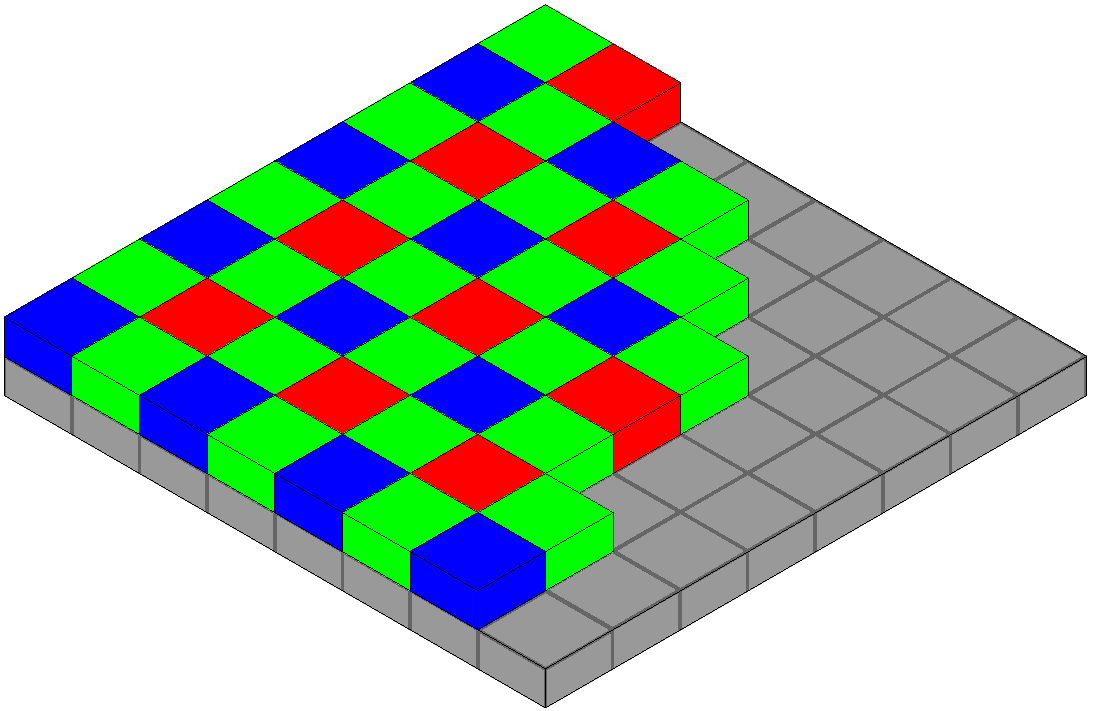
\psfig{file=figures/Bayer_pattern_on_sensor.pdf,width =3in}
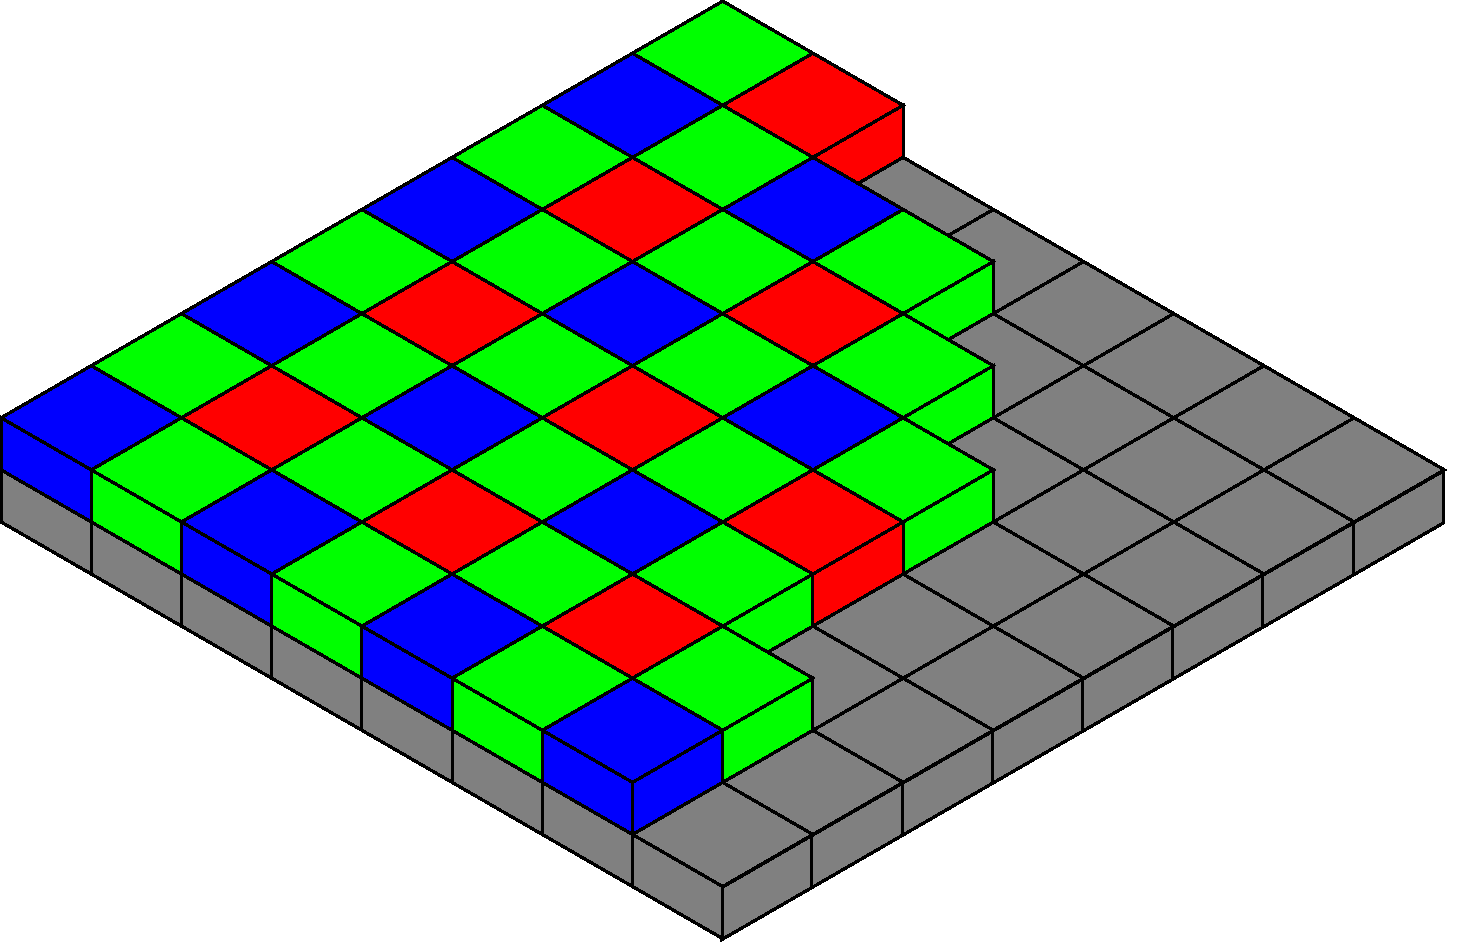
\includegraphics[width=\columnwidth]{20190404183627!Bayer_pattern_on_sensor}
\caption{A Bayer pattern on a sensor in isometric perspective.~\cite{wiki:BayerFilter}}
\label{fig:BayerPattern}
\end{figure}

\begin{figure*}[t]
\centering
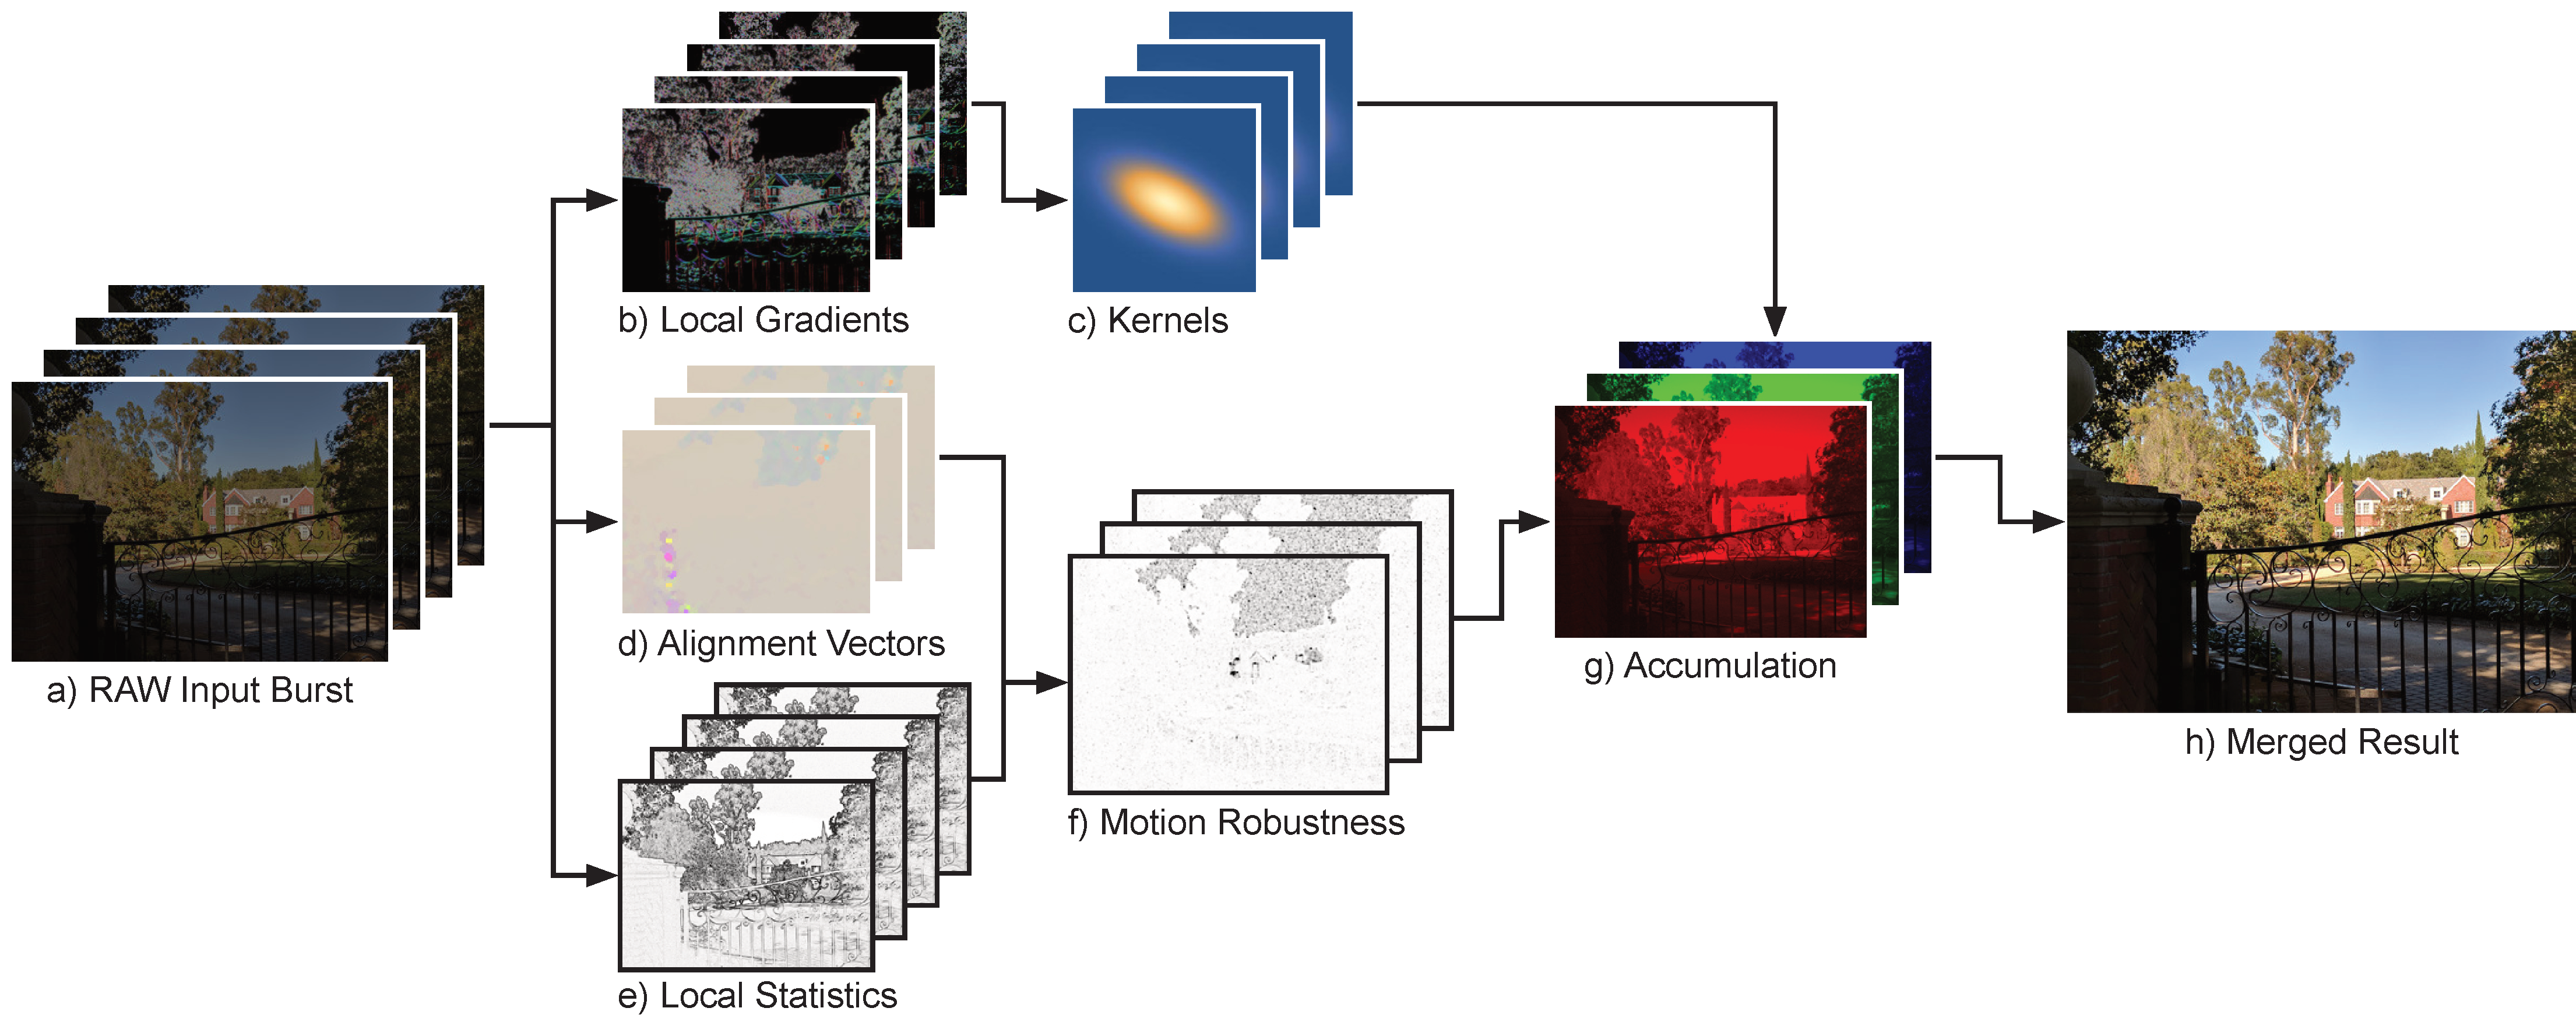
\includegraphics[width=\textwidth]{Wronski2019-figure-2}
\caption{An overview of the approach used by Wronski et al.~\cite{Wronski2019}. The initial burst of input frames (a) are aligned (d) to a base frame. The local features in the frames (b) are used to create kernels (c) (Section~\ref{sec:kernelReconstruction}) which are used along with the motion robustness model (f) (Section~\ref{sec:robustnessModel}) to combine (g) the frames separately for each color channel. The final image (h) is produced by normalizing the results of each channel.}
\label{fig:Wronski2019Fig2}
\end{figure*}

\pagebreak

\subsection{Burst Photography}
\label{sec:background:burstPhotography}

An image processing pipeline refers to the process the raw data from a camera sensor goes through to be turned into the final image file that can be displayed and shared. 
Most smartphones use a burst processing pipeline for their cameras. Generally, burst processing involves taking a series of exposures and merging them together to form the final image. Most smartphones operate in a \emph{zero-shutter lag} mode by default. In this mode, raw frames (the full unprocessed sensor output) are continuously captured to a temporary area in memory while the camera app is open. When the user presses the shutter button, several of the most recent frames are sent to the camera processing pipeline to be merged.

Both of the approaches in this paper build on the end-to-end burst processing pipeline from Hasinoff et al. \cite{Hasinoff2016} which used bursts of constant low-exposure frames to increase dynamic range and signal-to-noise ratio. It specifically uses under-exposed frames to reduce motion blur.

\subsection{Bayer Filters}
\label{sec:background:bayerFilter}

A Bayer filter is a type of color filter array (CFA). CFAs are needed because the light sensing components in a digital image sensor can only detect the presence of light and not what specific color it is. The majority of digital image sensors in digital cameras and phones use a Bayer filter mosaic pattern to arrange RGB color filters on the sensor (Figure~\ref{fig:BayerPattern}). The pattern consists of 50\% green, 25\% red, and 25\% blue pixels. This ratio emulates the color sensitivity of the human eye, which is more sensitive to green than it is to blue and red. Due to this pattern on the sensor, the raw output of a digital camera also has each pixel filtered to only red, green, or blue and a demosaicing algorithm must be used to interpolate the other values for each pixel.~\cite{wiki:BayerFilter}



\subsection{Demosaicing and Aliasing}
\label{sec:background:demosaicing}

A demosaicing algorithm reconstructs a full color image from the separate pixels that have been filtered with a CFA to just one channel: red, green, or blue \cite{wiki:Demosaicing}. There are many methods for this; the simplest ones interpolate the values for the other two color channels of a given pixel based on nearby pixels from the CFA image of those colors.

This process means two-thirds of the final image is reconstructed from the available data. The demosaicing process may introduce various artifacts in the final image due to aliasing, an effect that happens when the camera sensor is unable to correctly represent the patterns and details present in a scene due to its resolution. One type of artifact this causes are Moiré patterns, a type of interference pattern.~\cite{blog:Wronski2018}


\subsection{Super-resolution}
\label{sec:background:superResolution}

Super-resolution is any technique which increases the resolution of an image. While there are techniques that work on a single image, we will focus on using multiple frames for super-resolution. To do this each frame must have some new information to contribute to the final image.
This is achieved by capturing multiple aliased input frames that are sampled at different subpixel offsets, meaning the individual pixel points in each frame capture a different sample of the area the pixel represents~\cite{Wronski2019}. 


\subsection{Kernels}
\label{sec:background:kernels}

A kernel (or convolution matrix) in image processing refers to a small matrix that is used to apply effects like blurring or to detect features in an image, such as edges. The kernel is applied by doing a convolution, adding each pixel of the image to its local neighbors, weighted by the kernel. \cite{wiki:kernel}

For example, the following applies a kernel (the first matrix) to an image piece (the second matrix):
\begin{equation*}
\begin{bmatrix}
a & b & c \\
d & e & f \\
g & h & i
\end{bmatrix}
*
\begin{bmatrix}
1 & 2 & 3 \\
4 & 5 & 6 \\
7 & 8 & 9
\end{bmatrix}
\end{equation*}

The pixel in the center of the final image (coordinates $[2,2]$) would be this combination of the values of the image matrix weighted by the kernel matrix:
\begin{equation*}
(i \cdot 1)+(h \cdot 2)+(g \cdot 3)+(f \cdot 4)+(e \cdot 5)+(d \cdot 6)+(c \cdot 7)+(b \cdot 8)+(a \cdot 9)
\end{equation*}

% ----------------------------------------
\section{Handheld Super-resolution}
\label{sec:handheldSuperRes}

Wronski et al.~\cite{Wronski2019} introduced an algorithm that uses multiple shifted frames to produce higher resolution images from bursts of underexposed raw frames as part of the smartphone's imaging pipeline. The algorithm is able to directly use Bayer raw frames and removes the need for an explicit demosaicing step in the pipeline. It uses natural hand motion and is efficient enough to work in the background on smartphones. This algorithm is used as the merging algorithm in the camera pipeline of the Google Pixel 3 and newer and is what allows for the Pixel's ``super-res zoom" feature. This section provides an overview and some results of the algorithm by Wronski et al.~\cite{Wronski2019}.

\subsection{Algorithm Overview}

\begin{figure*}
\centering
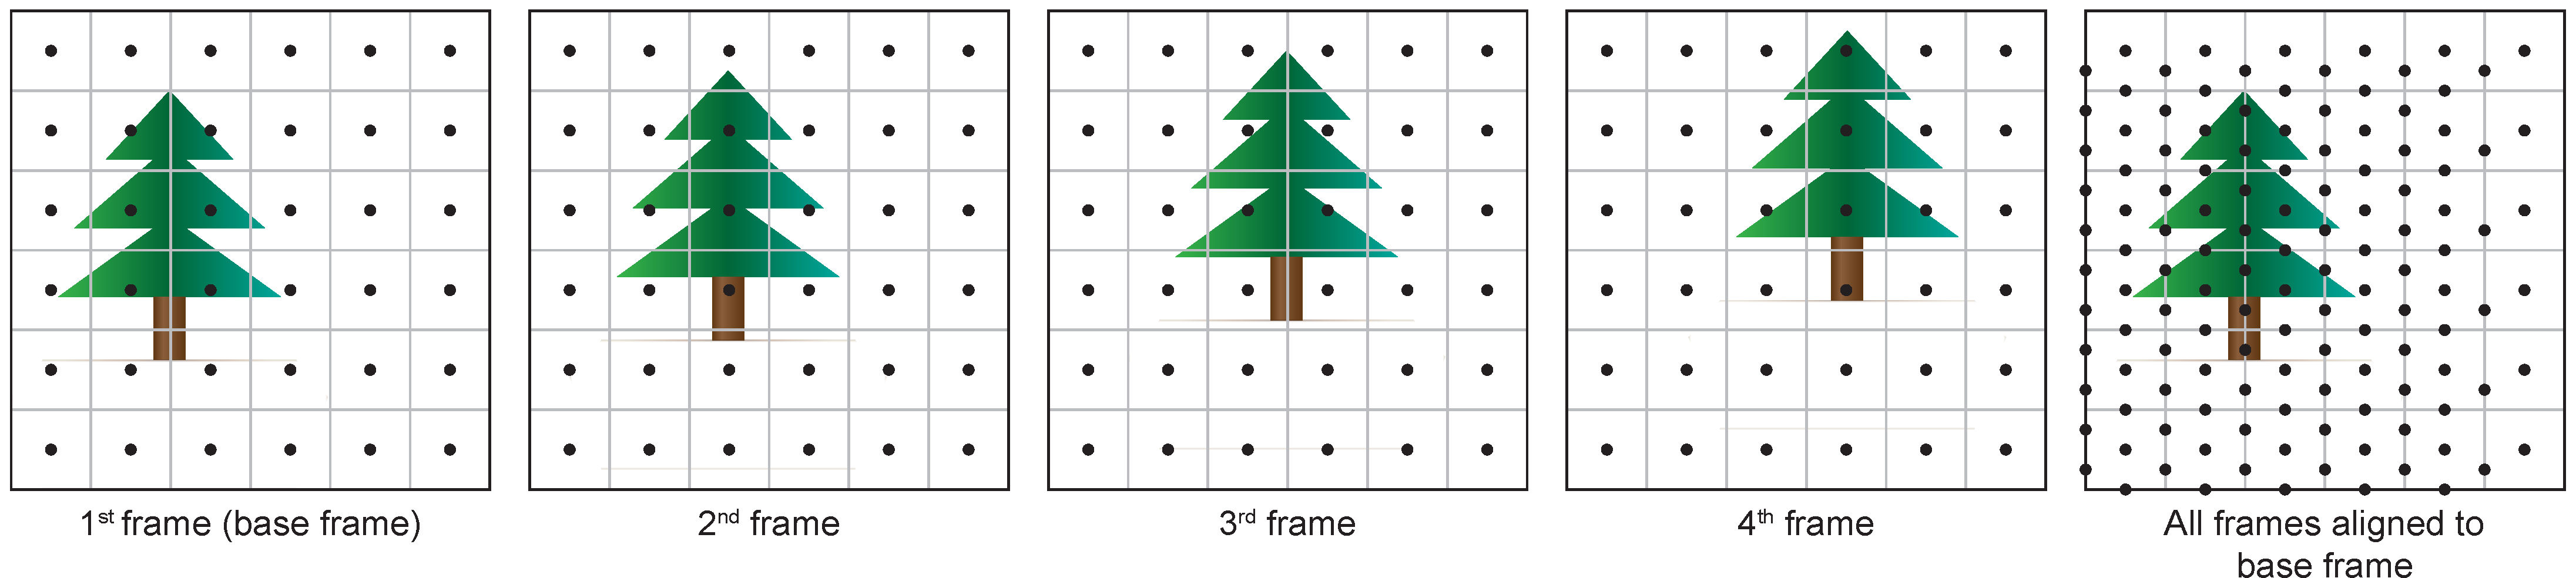
\includegraphics[width=\textwidth]{Wronski2019-figure-4}
\caption{An illustration of subpixel displacements from a burst of four frames with linear hand motion. Each frame is offset by half a pixel on the x-axis and a quarter pixel on the y-axis from the last frame. After alignment, the pixel centers (black dots) uniformly cover the image with greater density than a single frame.~\cite{Wronski2019}}
\label{fig:Wronski2019Fig4}
\end{figure*}

The approach by Wronski et al., as shown in Figure~\ref{fig:Wronski2019Fig2}, is a process that starts with the the acquisition of a burst from the continuous ring buffer of raw frames in the phone's camera application. Next, a single frame is chosen and the rest are aligned to it using a refined version of the algorithm by Hasinoff et al.~\cite{Hasinoff2016}.
% TODO: elaborate on the alignment algorithm
Each frame's local contributions are estimated through kernel regression (Section~\ref{sec:kernelReconstruction}) and accumulated across a whole burst for each of the three color planes. This involves the kernel shapes being adjusted based on estimated local gradients and, at the same time, the sample contributions are adjusted weighted based on a statistical robustness model (Section~\ref{sec:robustnessModel}).


The final RGB image is obtained by normalizing the accumulated contributions for each of the three color planes and merging them together. This can then be sent to the rest of the imaging pipeline.

\subsection{Hand Movement Based Super-resolution}

One of the important conditions for multi-frame super-resolution is that the input contains multiple images that are sampled at different subpixel offsets. When someone is holding an object there is a natural and involuntary slight hand movement present. Wronski et al. analyzed hand movement in a set of 86 bursts captured by 10 different users during regular smartphone photography using the rotational measurements from the phone's gyroscope. They determined this periodic, random movement while the camera is capturing a burst frames provides sufficient subpixel coverage to create a super-resolution image.

\begin{figure}
\centering
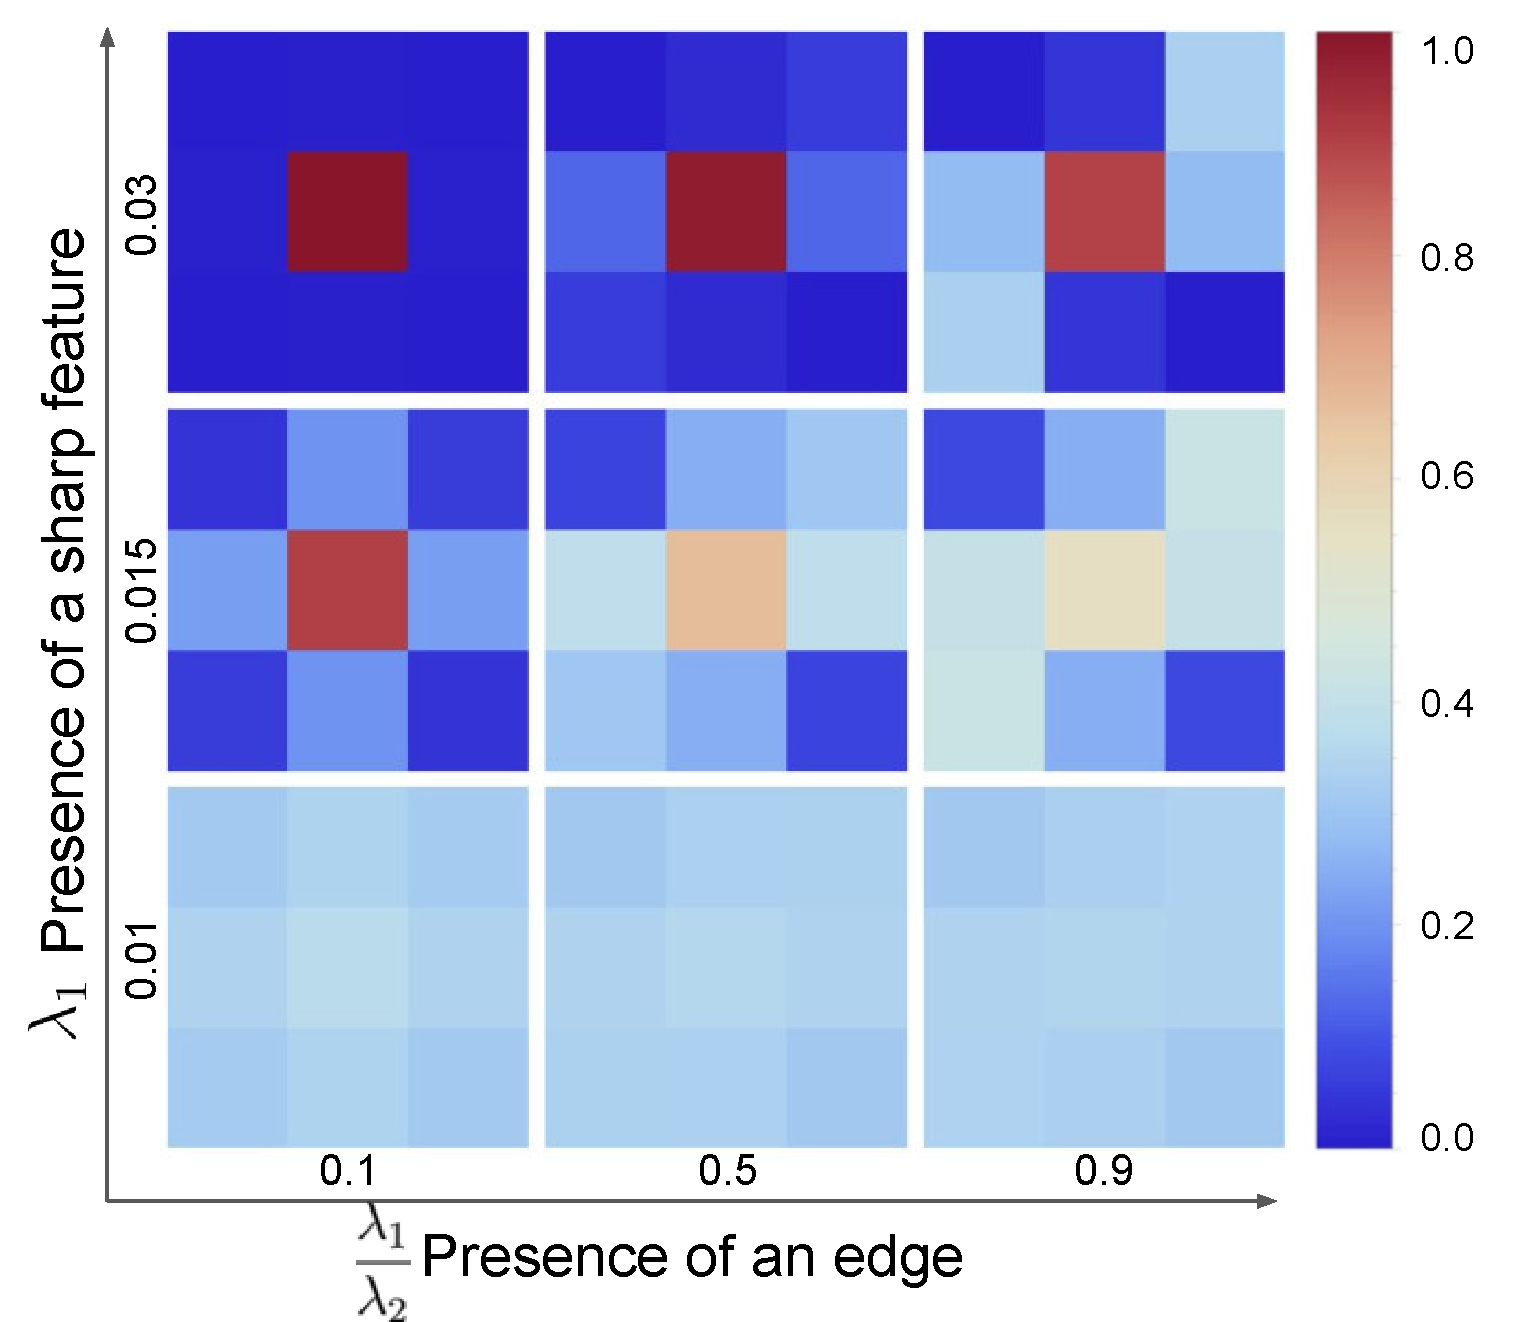
\includegraphics[width=19pc]{figures/Wronski2019-figure-8.pdf}
\caption{Plots of relative weights as a function of local features. The scale on the right indicates the weight given to each pixel in the $3\times 3$ neighborhood.~\cite{Wronski2019}}
\label{fig:Wronski2019Fig8}
\end{figure}

\pagebreak

\subsection{Kernel Reconstruction}
\label{sec:kernelReconstruction}

The core idea of the algorithm is considering the pixels of multiple raw frames with hand motion as randomly offset, aliased, and noisy measurements of three original continuous signals, one for each color channel. The algorithm creates the final output image pixel-by-pixel. For each output pixel, it evaluates the local contributions to each of the three color channels from different input frames since each raw image pixel is specific to a single color channel. 

The process for each pixel in each color channel can be described as:
\begin{equation*}
C(x, y)=\frac{\sum_{n} \sum_{i} c_{n, i} \cdot w_{n, i} \cdot \hat{R}_{n}}{\sum_{n} \sum_{i} w_{n, i} \cdot \hat{R}_{n}}
\end{equation*}

\begin{description}
  \item[$(x,y)$] refers to the coordinates of the pixel. 
  \item[$\sum_{n}$] is a sum over all contributing frames.
  \item[$\sum_{i}$] is the sum over samples (pixels) in a local $3\times 3$ neighborhood centered on the target pixel.
  \item[$c_{n, i}$] is the value of the individual pixel at frame $n$ and sample $i$.
  \item[$w_{n, i}$] is the local sample weight for the pixel at frame $n$ and sample $i$, which is described below. 
  \item[$\hat{R}_{n}$] is the local motion robustness score at $(x,y)$ described in Section~\ref{sec:robustnessModel}.
\end{description}

The local pixel weights ($w_{n, i}$) come from a kernel which is calculated for the $3\times 3$ neighborhood around the pixel at $(x,y)$.\footnote{Specifically a 2D unnormalized anisotropic Gaussian radial basis function kernel.} It produces a $3\times 3$ matrix of values between 0 and 1 taking into account edges and sharp features in the local area. These weights determine how much each pixel in the $3\times 3$ area will contribute to the target pixel for that frame. An example of the matrices that result from the kernel function can be seen in Figure~\ref{fig:Wronski2019Fig8}. Here the presence of a sharp feature produces a matrix where more emphasis is put on just the center pixel.

\pagebreak

\subsection{Motion Robustness}
\label{sec:robustnessModel}

\begin{figure}
\centering
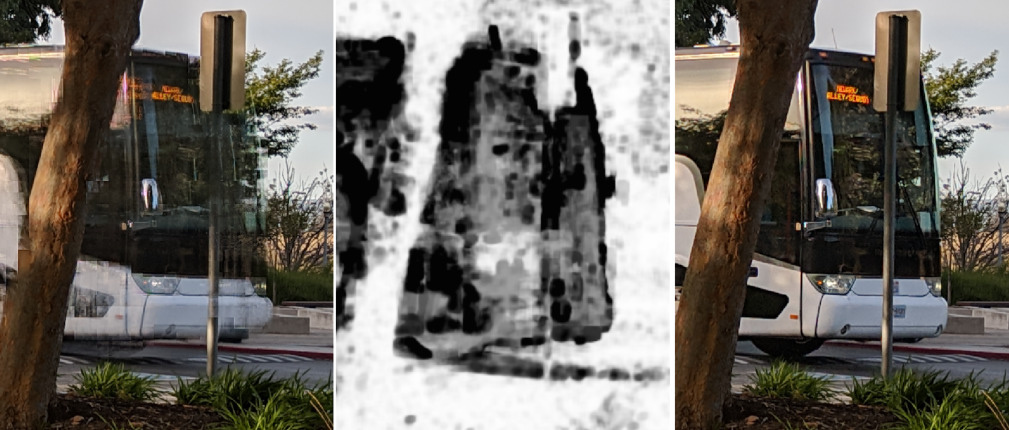
\includegraphics[width=\columnwidth]{figures/wronski2019-figure-9-95quality.jpg}
\caption{A photograph of a moving bus: \textbf{Left}: Without a motion robustness model there are alignment errors and occlusions that result in tiling and ghosting artifacts. \textbf{Middle}: The robustness mask produced by the robustness model. White regions are those with all frames contributing to the final merged image and darker regions are those with a lower number of contributing frames. \textbf{Right}: The result of using the robustness model when merging frames. \cite{Wronski2019}}
\label{fig:Wronski2019Fig9}
\end{figure}

 
It is difficult to reliably align the sequence of images in a burst and even assuming a perfect alignment, changes in the scene and occlusion would still result in some areas of the scene being poorly represented in many frames of the burst. This needs to be taken into account to prevent severe artifacting (Figure~\ref{fig:Wronski2019Fig9} Left). To combine frames robustly, a confidence level is assigned to the local neighborhood of each pixel; the map of these confidences is called a \emph{robustness map}.

This confidence level is assigned by computing the standard deviation in the image and a color difference between the base frame and the aligned input frame. Regions of this frame with differences smaller than the local standard deviation and those that are close to a pre-defined fraction of the spatial standard deviation will be merged while larger differences are likely non-aligned motion and are discarded.

An example of what this can be seen in the middle image of Figure~\ref{fig:Wronski2019Fig9}, where the dark areas have a lower robustness value and the lighter areas have a greater robustness value.

\subsection{Results}



Wronski et al. used a variety of methods, both numerical and visual, to evaluate their algorithm and compare it with other demosaicing, merging, and super-resolution techniques. They also compared their method as part of a full camera pipeline to that of Hasinoff et al.~\cite{Hasinoff2016}. Figure~\ref{fig:wronskiResults} shows one of these comparisons.

\begin{figure}
\centering
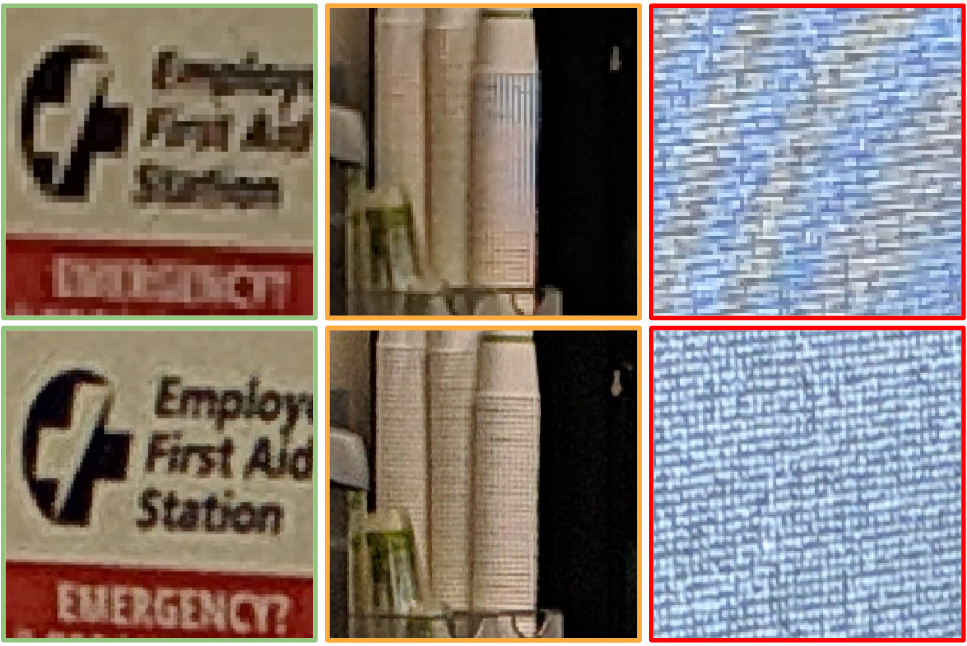
\includegraphics[width=\columnwidth]{figures/wronski2019-figure-1-100quality-crop.jpg}

\caption{A comparison of the traditional frame merging approach (\textbf{top}) and the approach by Wronski et al. (\textbf{bottom}). The super resolution merge algorithm improves sharpness and detail while eliminating the 
Moiré aliasing artifacts (false color banding) seen in the third (\textbf{red}) frame.~\cite{Wronski2019}}


\label{fig:wronskiResults}
\end{figure}

% ----------------------------------------
\section{Handheld Low Light Photography}
\label{sec:handheldLowLight}

Liba et al.~\cite{Liba2019} introduce a system for capturing photos in very low light that produces improved color and less noise. This system is used for the ``Night Sight" feature on Google Pixel phones.
The system builds on the existing burst pipeline (from Hasinoff et al.~\cite{Hasinoff2016}) and uses the burst merging algorithm from Wronski et al.~\cite{Wronski2019} with modifications to improve low-light photography. It uses a \emph{positive-shutter-lag} mode where the camera waits until the shutter button is pressed to capture the burst of frames. This is used rather than the \emph{zero-shutter-lag} mode used for daylight photography to allow for longer exposures.

The main improvements to the camera pipeline from this research are the use of ``motion metering" (Section~\ref{sec:motionMetering}) to calculate the exposure settings for each frame based on predicted motion in the scene and camera, a learning-based low-light optimized auto white balance algorithm (Section~\ref{sec:autoWhiteBal}), and tone mapping (Section~\ref{sec:toneMapping}) to produce better colors in low light.

\subsection{Motion Metering}
\label{sec:motionMetering}

\begin{figure}
\centering
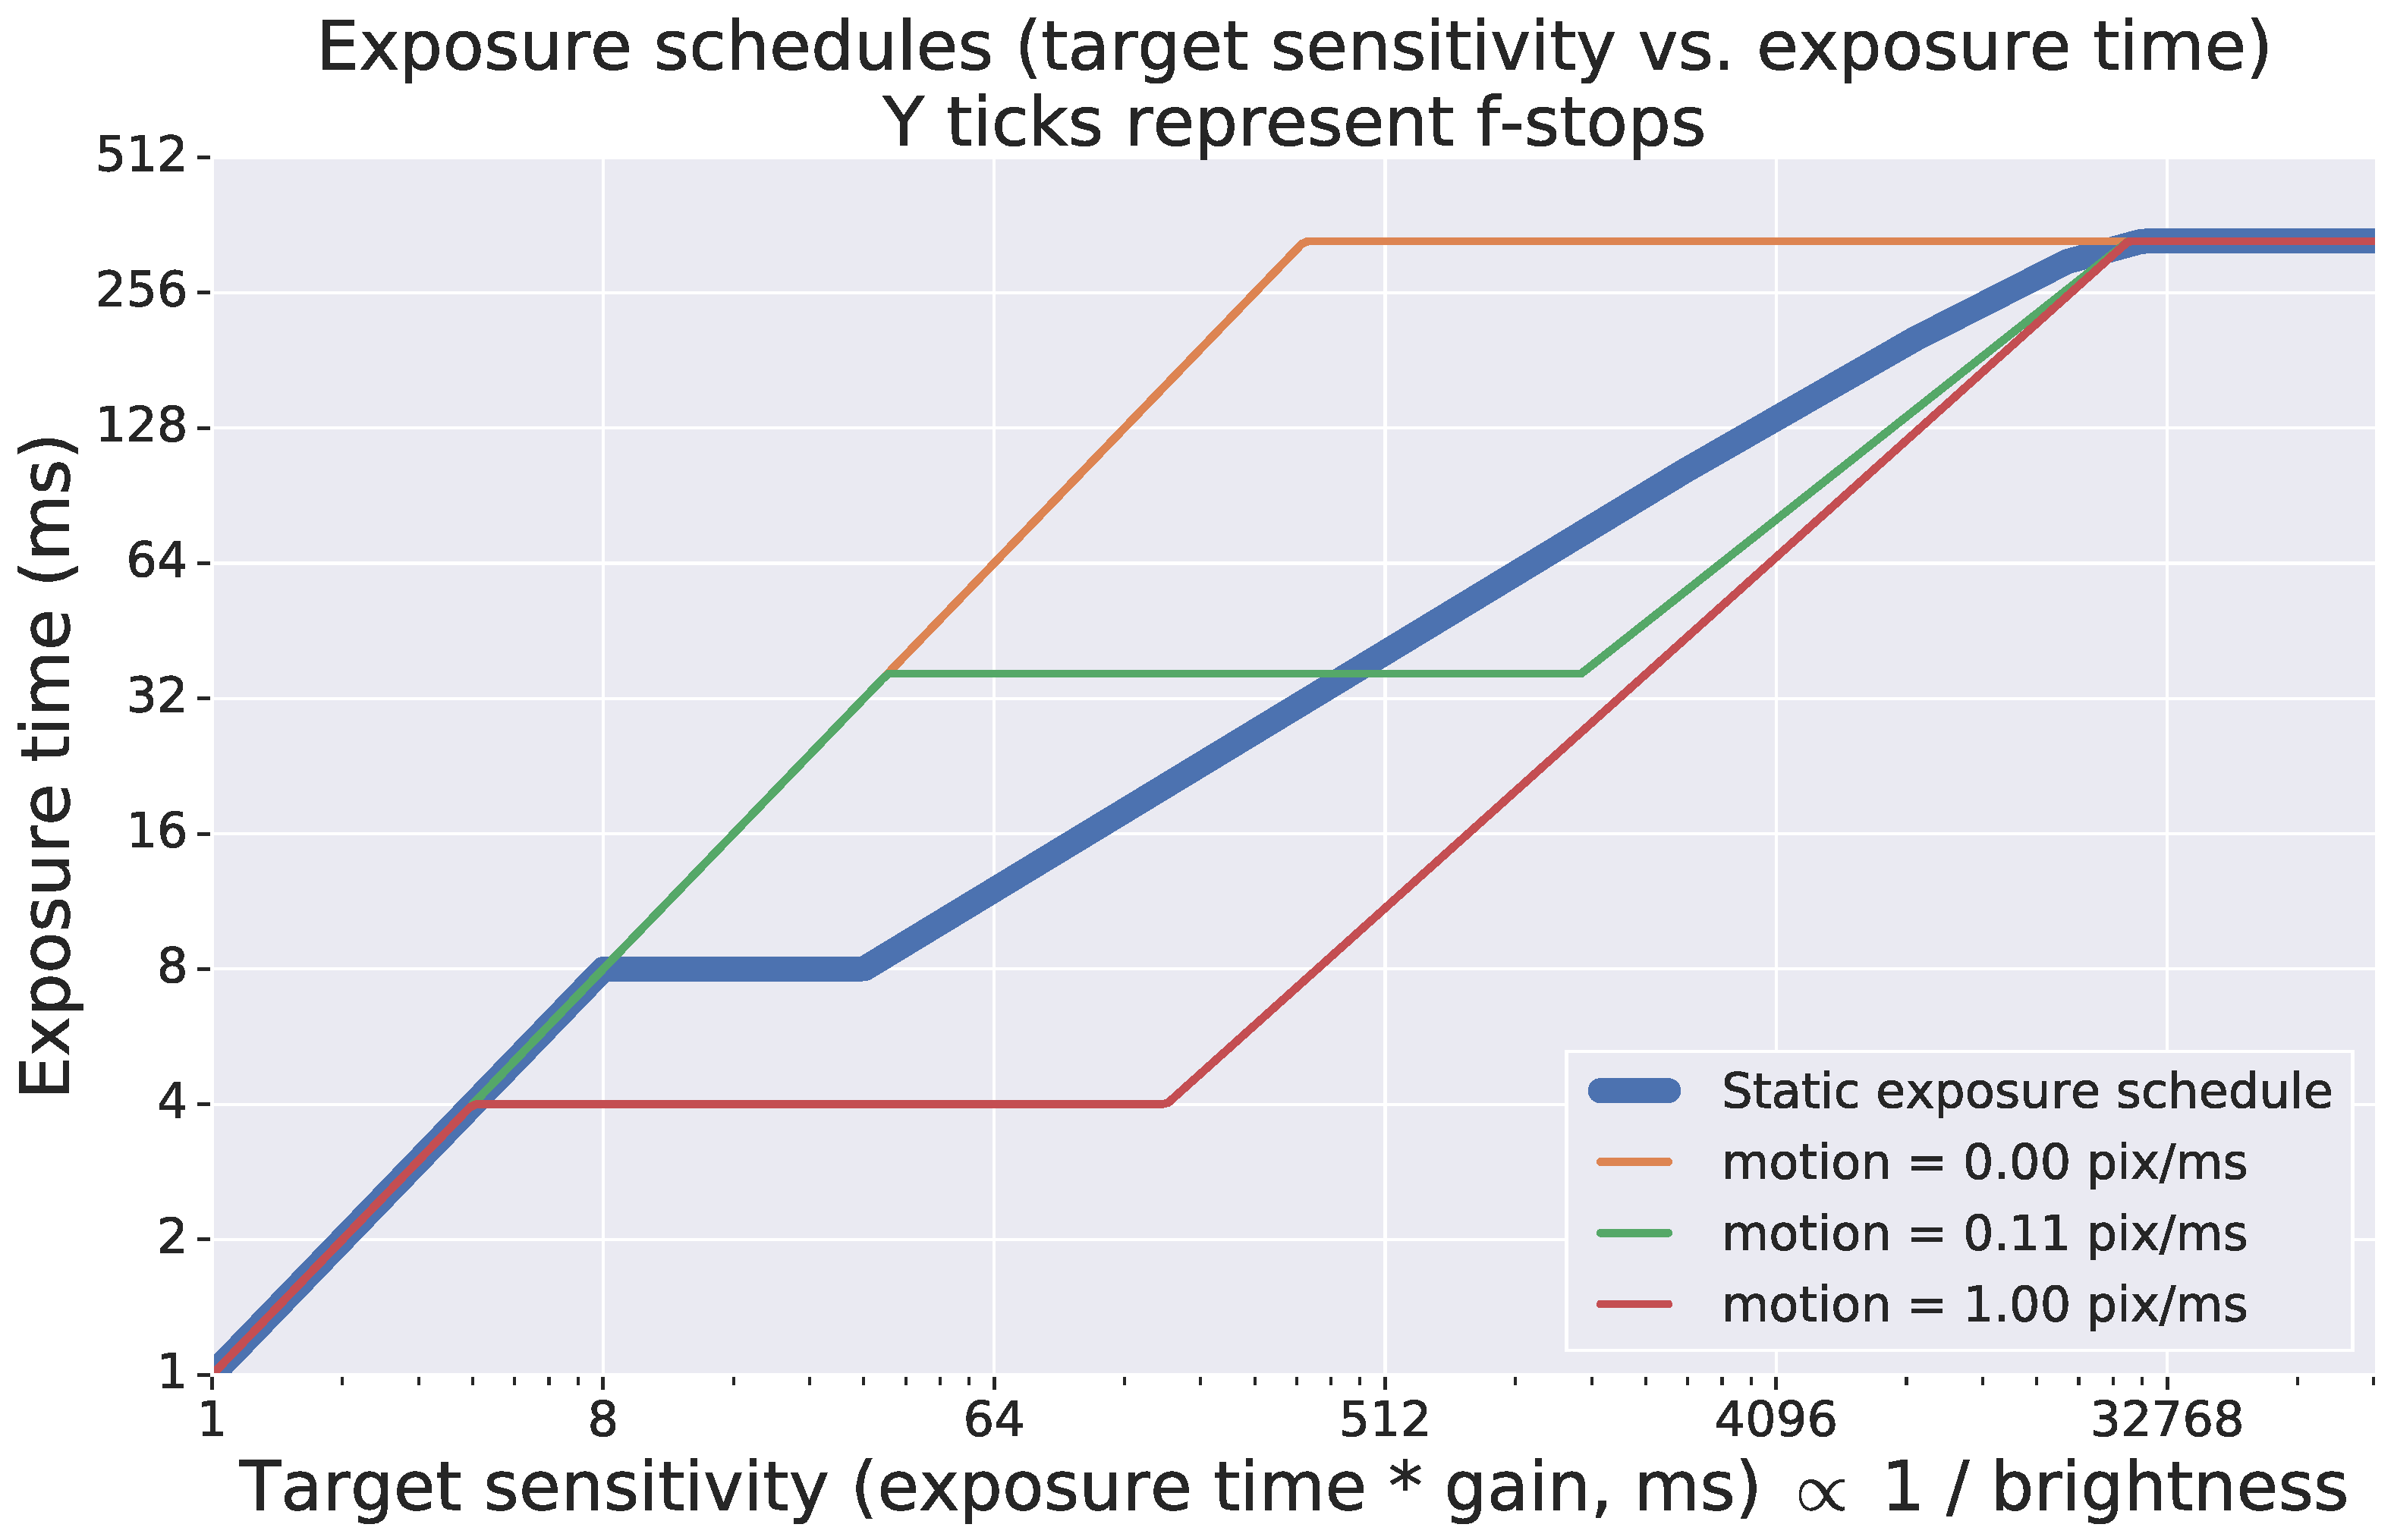
\includegraphics[width=\columnwidth]{figures/liba2019-figure-7.pdf}
\caption{A traditional static exposure schedule compared to the dynamic exposure schedule of Liba et al. at various levels of motion.~\cite{Liba2019}}
\label{fig:exposure}

\end{figure}

When capturing a burst of images on a smartphone, the exposure time and sensor gain (the sensitivity of the sensor to light, also known as ISO) needs to be selected for each frame. Liba et al. use the same strategy as in~\cite{Hasinoff2016} and capture all frames in the burst with the same exposure time and ISO. For effective low-light photography these settings need to be automatically selected within the constraints of keeping the total capture time low ($\leq$ 6 seconds) and the total number of frames within the device's memory limits.

This process consists of splitting the target sensitivity, which is based on the brightness of the scene, into exposure time and gain and calculating the number of frames with respect to the time and memory limits. The traditional method used in Hasinoff et al.~\cite{Hasinoff2016} uses a fixed ``exposure schedule" that simply keeps the exposure time low to limit motion blur. This method usually works well but can be improved for low-light photography.

The ``motion metering" described by Liba et al. selects the exposure time and gain by predicting future motion in the scene and motion of the camera itself. It produces a variable exposure schedule that varies based on the amount of motion detected (Figure~\ref{fig:exposure}). This is used to select longer exposures for scenes with no motion and shorter exposures for those with motion to reduce motion blur when needed and increase signal-to-noise ratio when possible.

Additionally, experienced photographers often brace their device against a surface or put it on a tripod in low light. Liba et al.'s motion metering system is able to use even longer exposures (up to 1 second) by detecting this using measurements from the device's gyroscope.

\subsection{Auto White Balance in Low Light}
\label{sec:autoWhiteBal}

\begin{figure}
\centering
\begin{subfigure}{9.8pc}
\centering
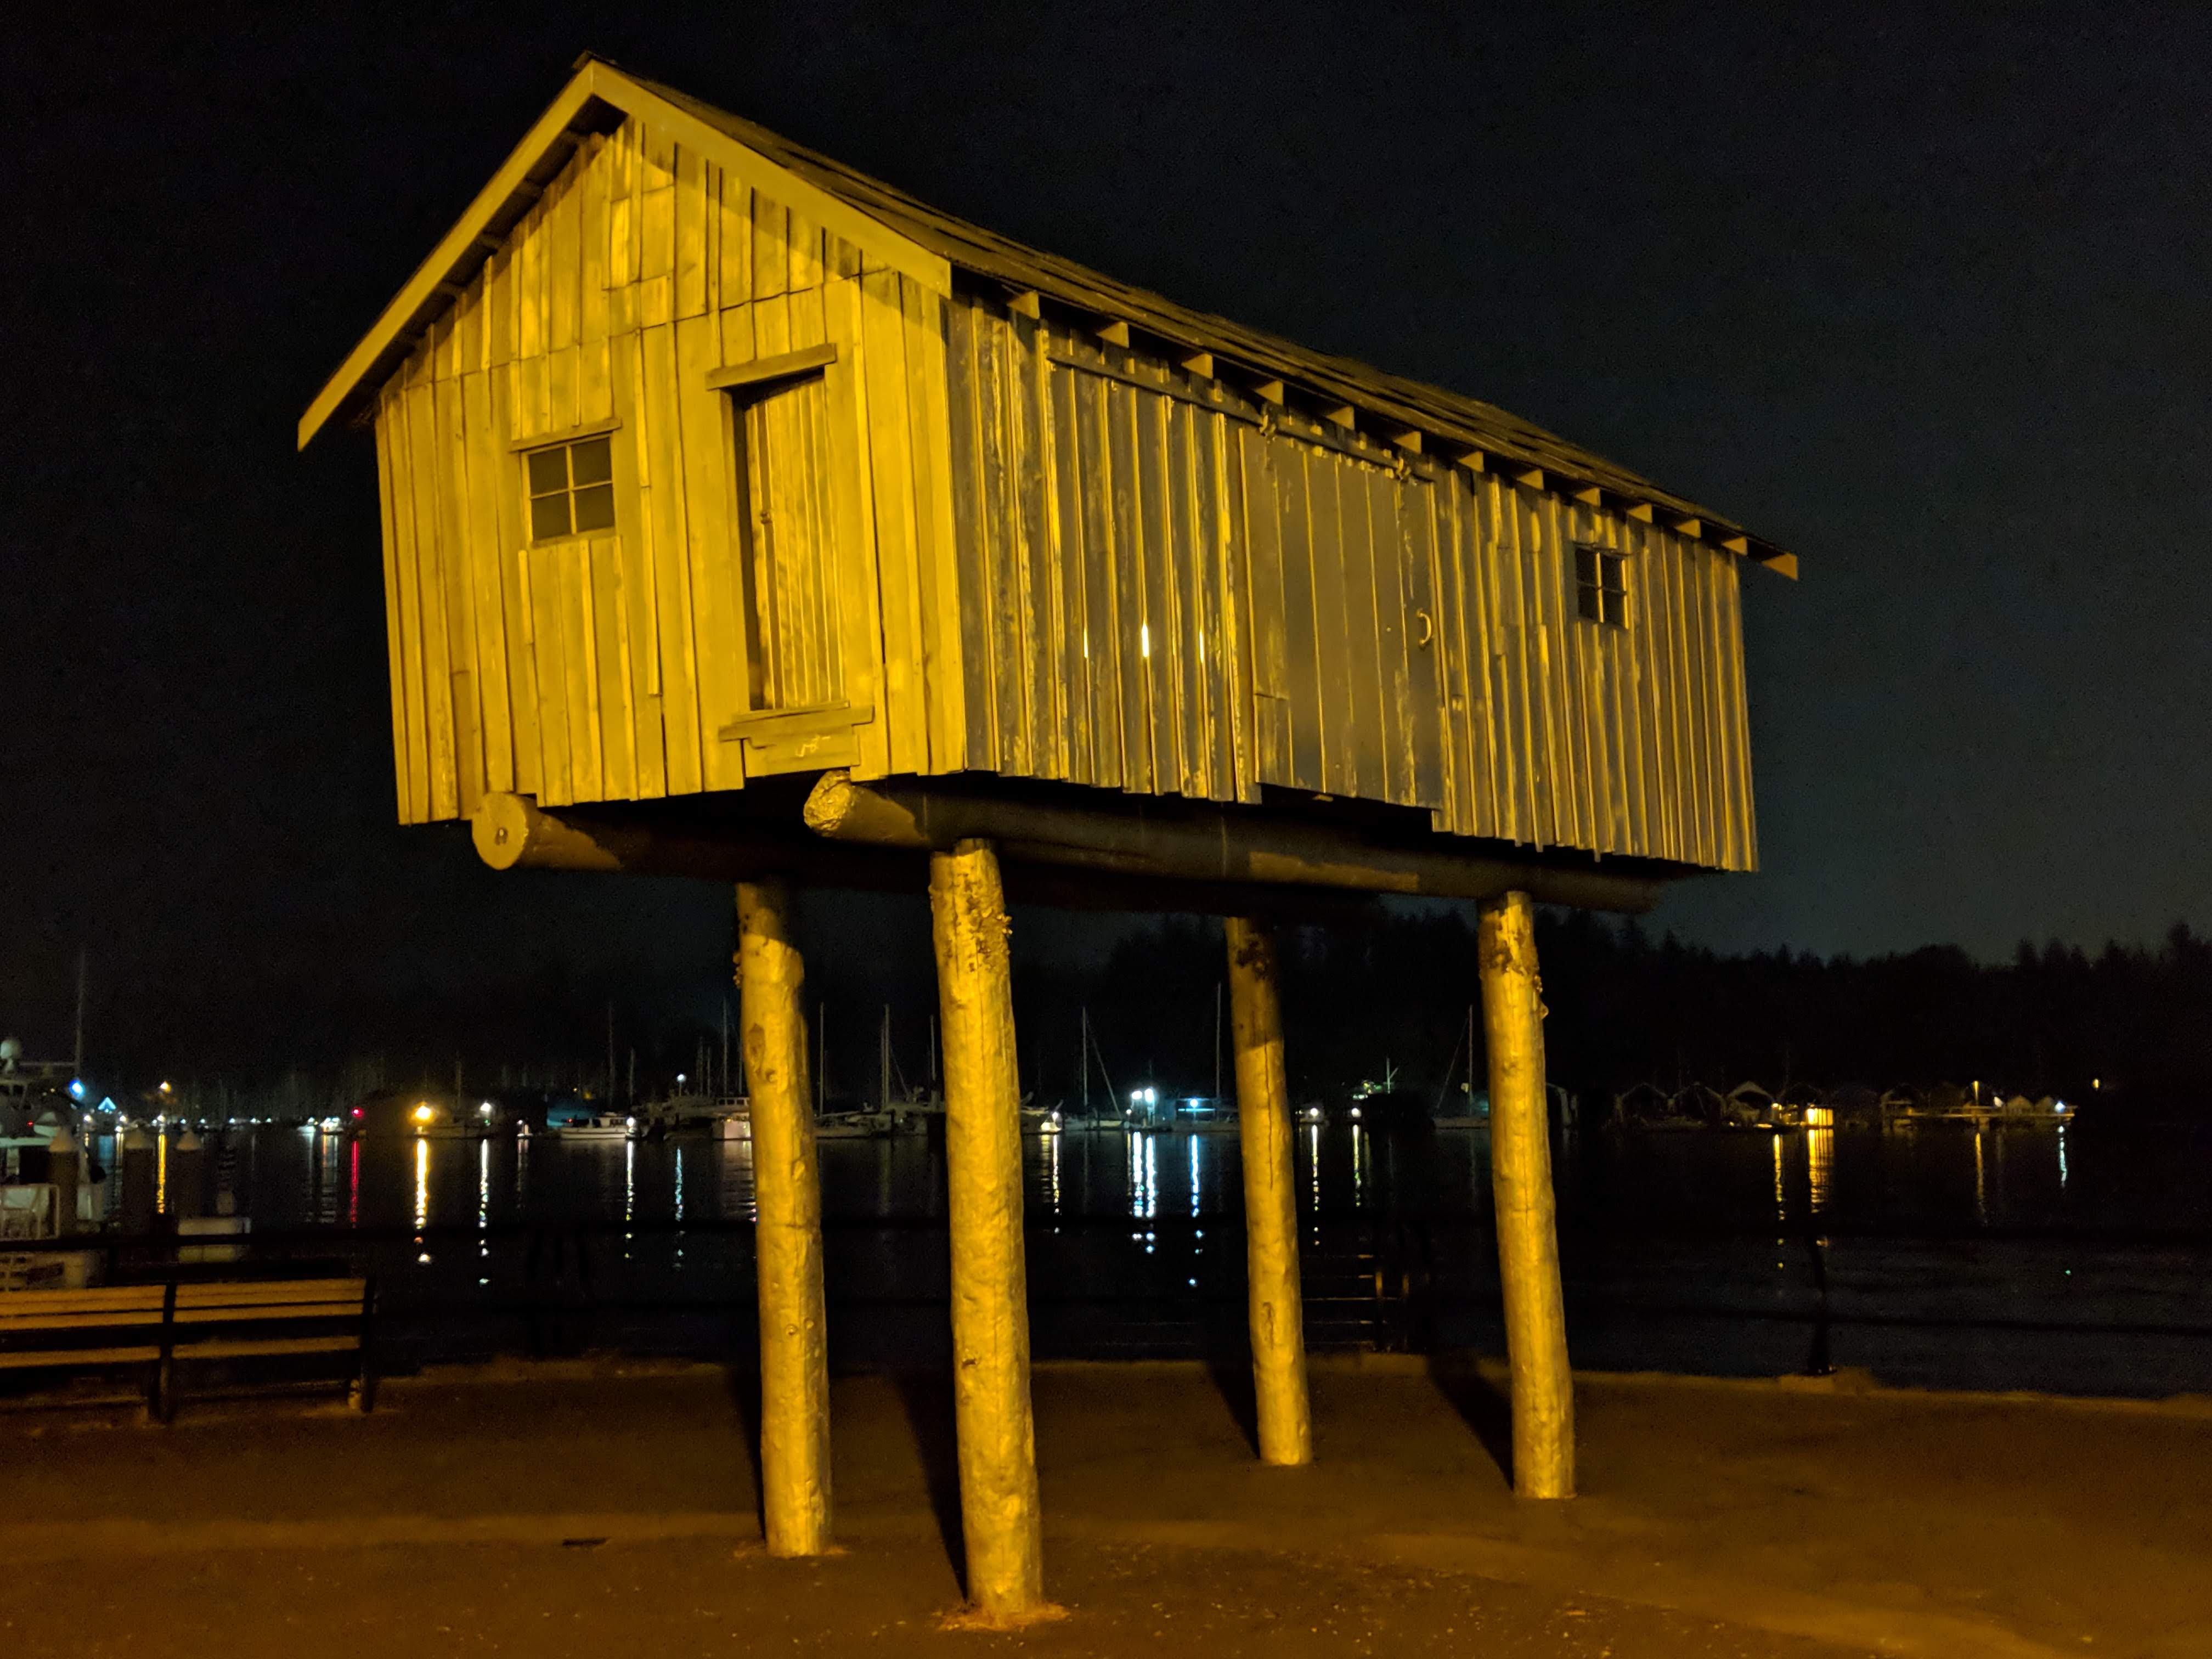
\includegraphics[width=9.8pc]{figures/0GMA_20180814_233948_174_qc.jpg}
\caption{Pixel default AWB}
\label{fig:whitebalance:default}
\end{subfigure}
\begin{subfigure}{9.8pc}
\centering
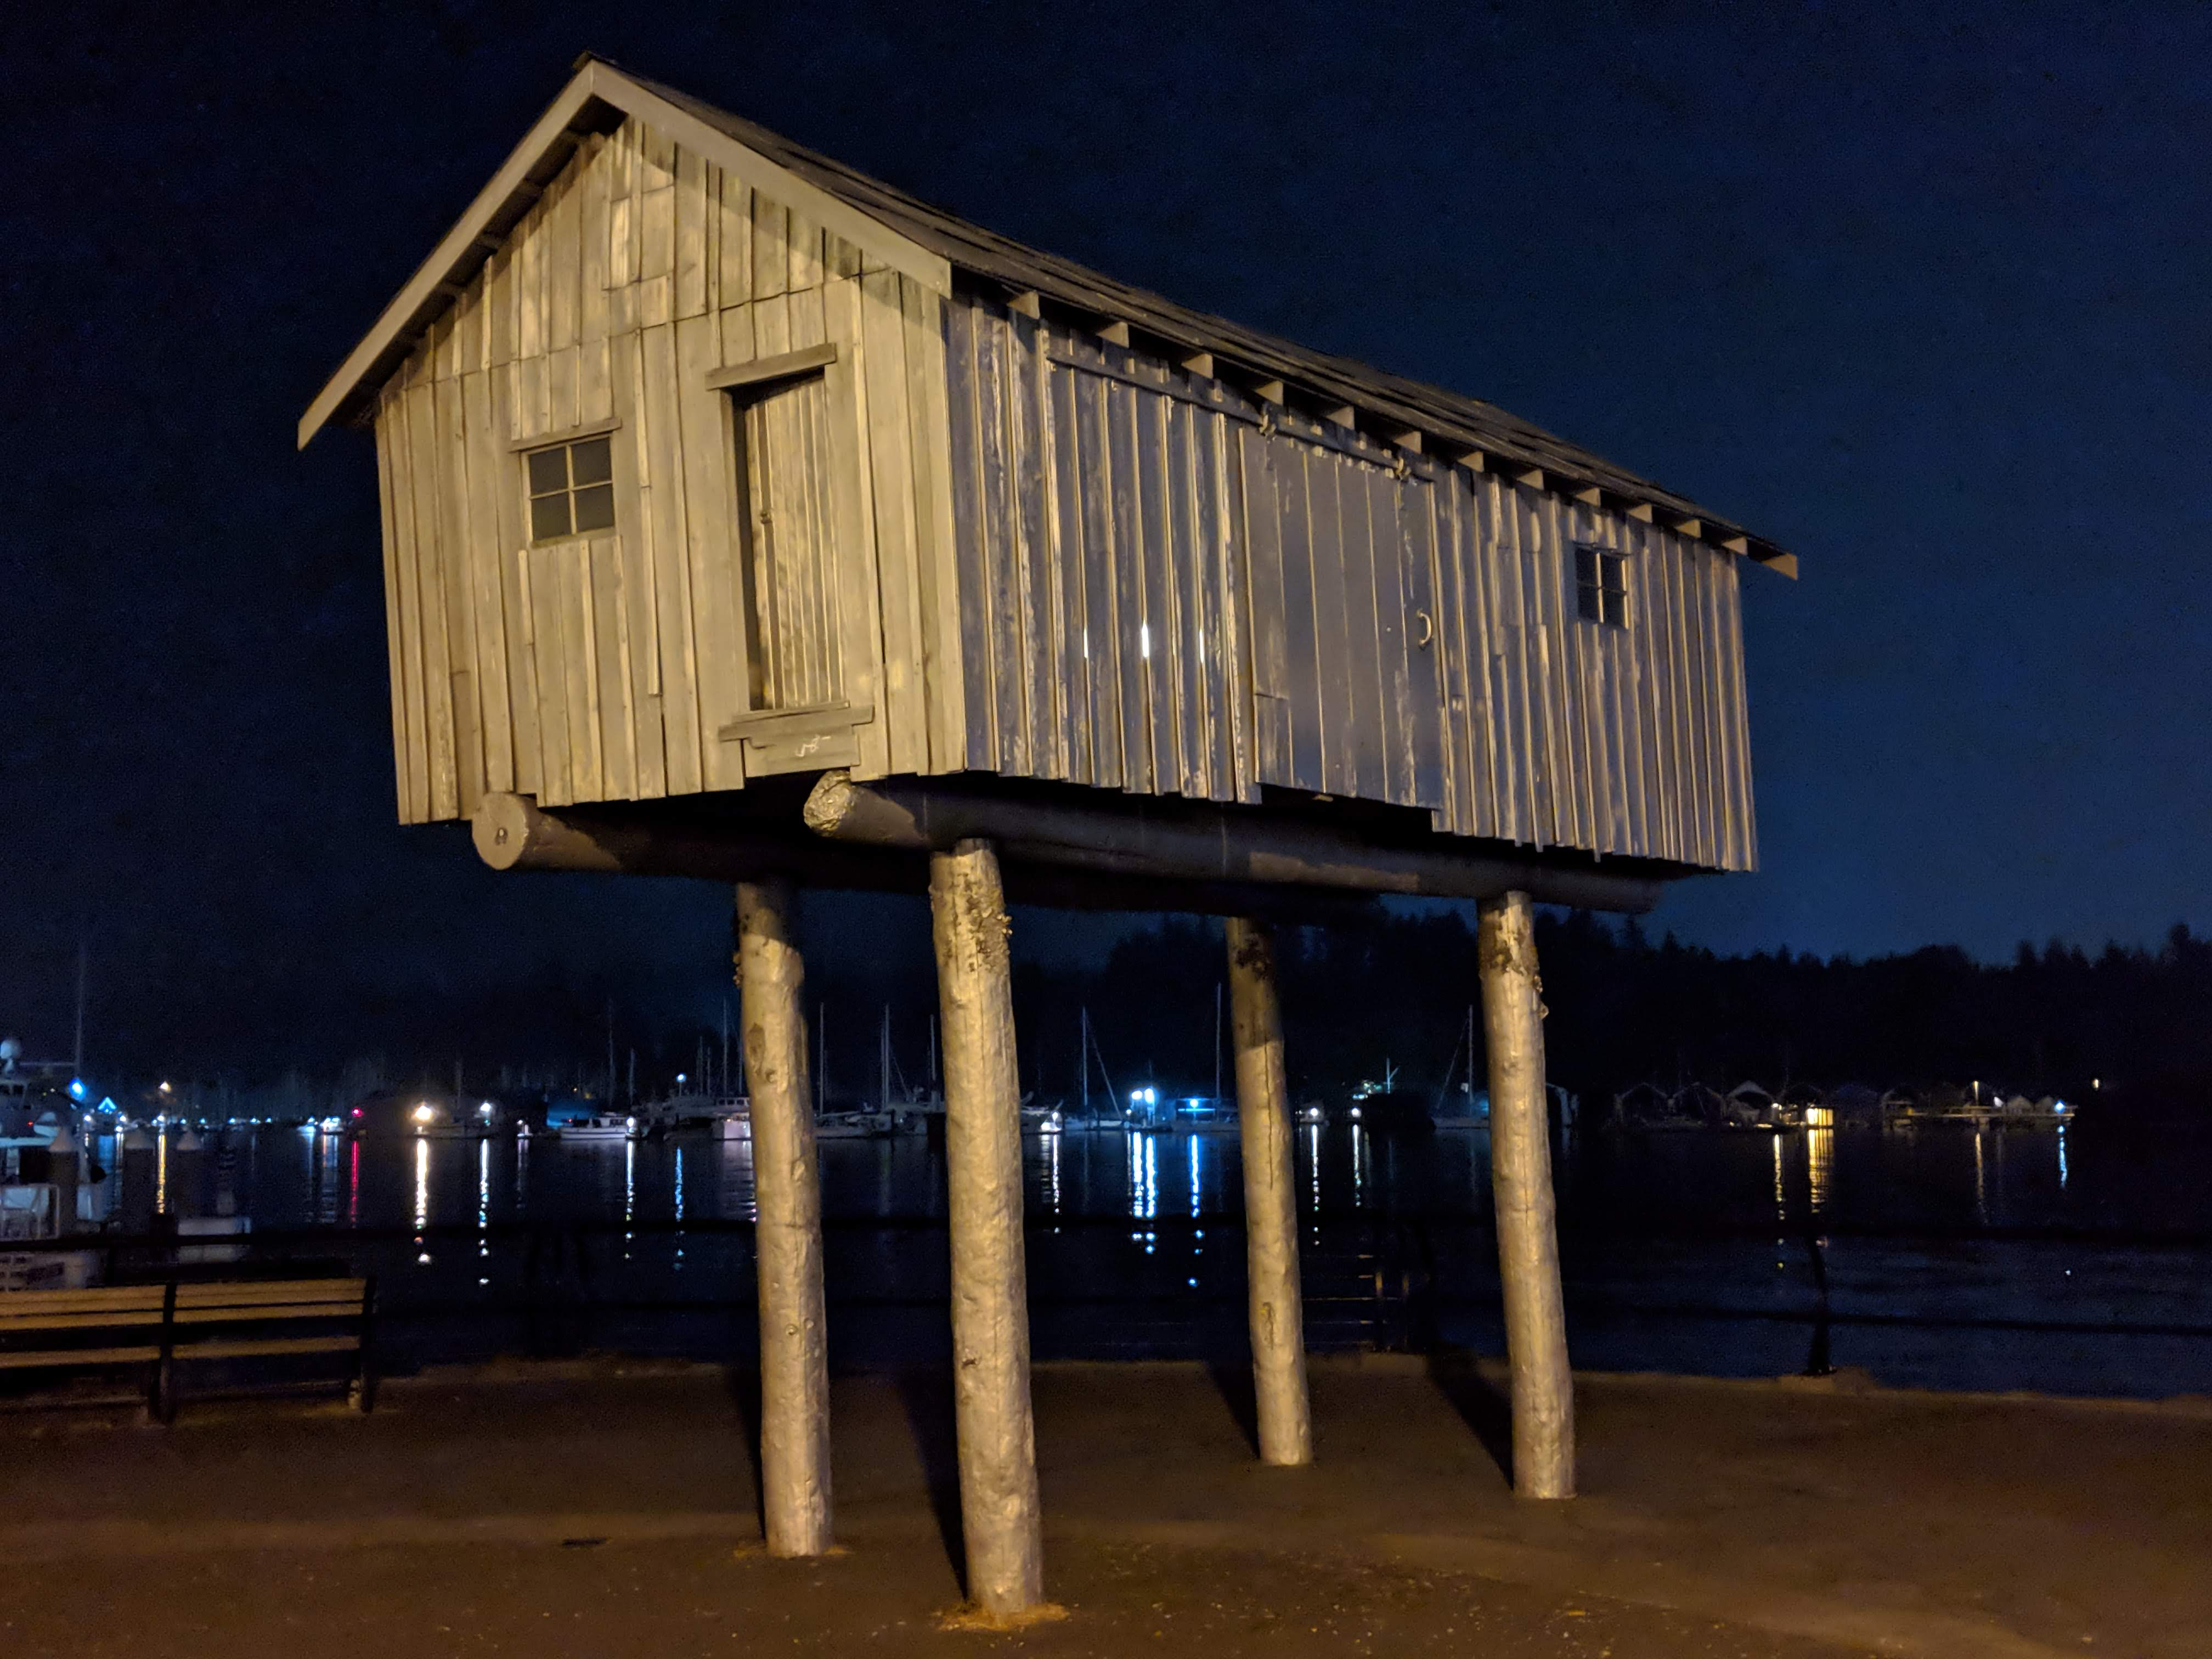
\includegraphics[width=9.8pc]{figures/0GMA_20180814_233948_174_gcam.jpg}
\caption{Liba et al.}
\label{fig:whitebalance:liba}
\end{subfigure}

\caption{A comparison of the default implementation of FFCC in the Pixel's camera and the low-light optimized version by Liba et al.~\cite{blog:Levoy2018}}


\label{fig:whitebalance}
\end{figure}


Humans perceive color correctly even when objects are lit with colored light, an ability called color constancy. This perception can break down when a photograph is taken under one type of light and viewed under different light, the image can look tinted (Figure~\ref{fig:whitebalance:default}).
Cameras correct for this by determining the color of the majority of the illumination in the scene and correcting the colors in the image such that they appear to be lit by a neutral (white) illumination. 
This Automatic White Balance (AWB) step in the camera pipeline is important to produce a pleasing image. \cite{blog:Levoy2018}

The current best-performing color constancy algorithm is the machine learning based ``Fast Fourier Color Constancy" (FFCC) \cite{Barron2017}.
As described in this section, Liba et al. trained the FFCC algorithm with a new dataset and error metric to better handle challenging low-light scenes (Figure~\ref{fig:whitebalance}).

Liba et al. collected 5000 images using mobile devices of various scenes that demonstrate a range of light levels to be able to train their implementation of FFCC. To obtain better ground truth coloring for the training data they had real professional photographers manually white balance the images with the most ``aesthetically preferable" white balance for the scene rather than use a color checker or grey card to empirically measure the ``true" white balance.

Additionally, Liba et al. developed a new error metric for training the model that better deals with heavily tinted illuminants which are common in night scenes (like those from colorful neon lights). The issue with traditional error metrics in low light is that they are based on how well the algorithm recovers \emph{all} of the color channels of the illuminant. This works well for brighter scenes with close to white true illumination but in dark scenes with heavily tinted illuminants the white balanced image may contain pixel values where a single color channel's values are near zero for the whole image. Such an image would look the same under all possible transformations of that channel. 
When a color channel is ``missing" it can produce low accuracy results from the error metric. It is also unclear how to set the missing channels in the ground-truth illuminant data.

The existing error metric for color constancy looks at the error in appearance of a white patch in the image, but that idea doesn't work in heavily-tinted scenes with missing color channels so the improved error metric considers the appearance of an \emph{average} portion of the image under the recovered illumination. It is able to be less sensitive to errors in channels with lower mean values in the true image.

\begin{figure}
\centering
\includegraphics[trim={0 000 0 0}, clip=true, width=\columnwidth]{figures/Wright_of_Derby_The_Orrery}
\caption{ \emph{Philosopher Lecturing on the Orrery}, by Joseph Wright of Derby, 1766 \cite{file:theOrrery}. The artist depicts a dark scene with bright, colorful detail while still maintaining the nighttime aesthetic by increasing contrast, surrounding the scene in darkness, and keeping the shadow areas completely black.~\cite{blog:Wronski2018}}
\label{fig:theOrrery}
\end{figure}

\begin{figure}
\centering
\begin{subfigure}{6.5pc}
\centering
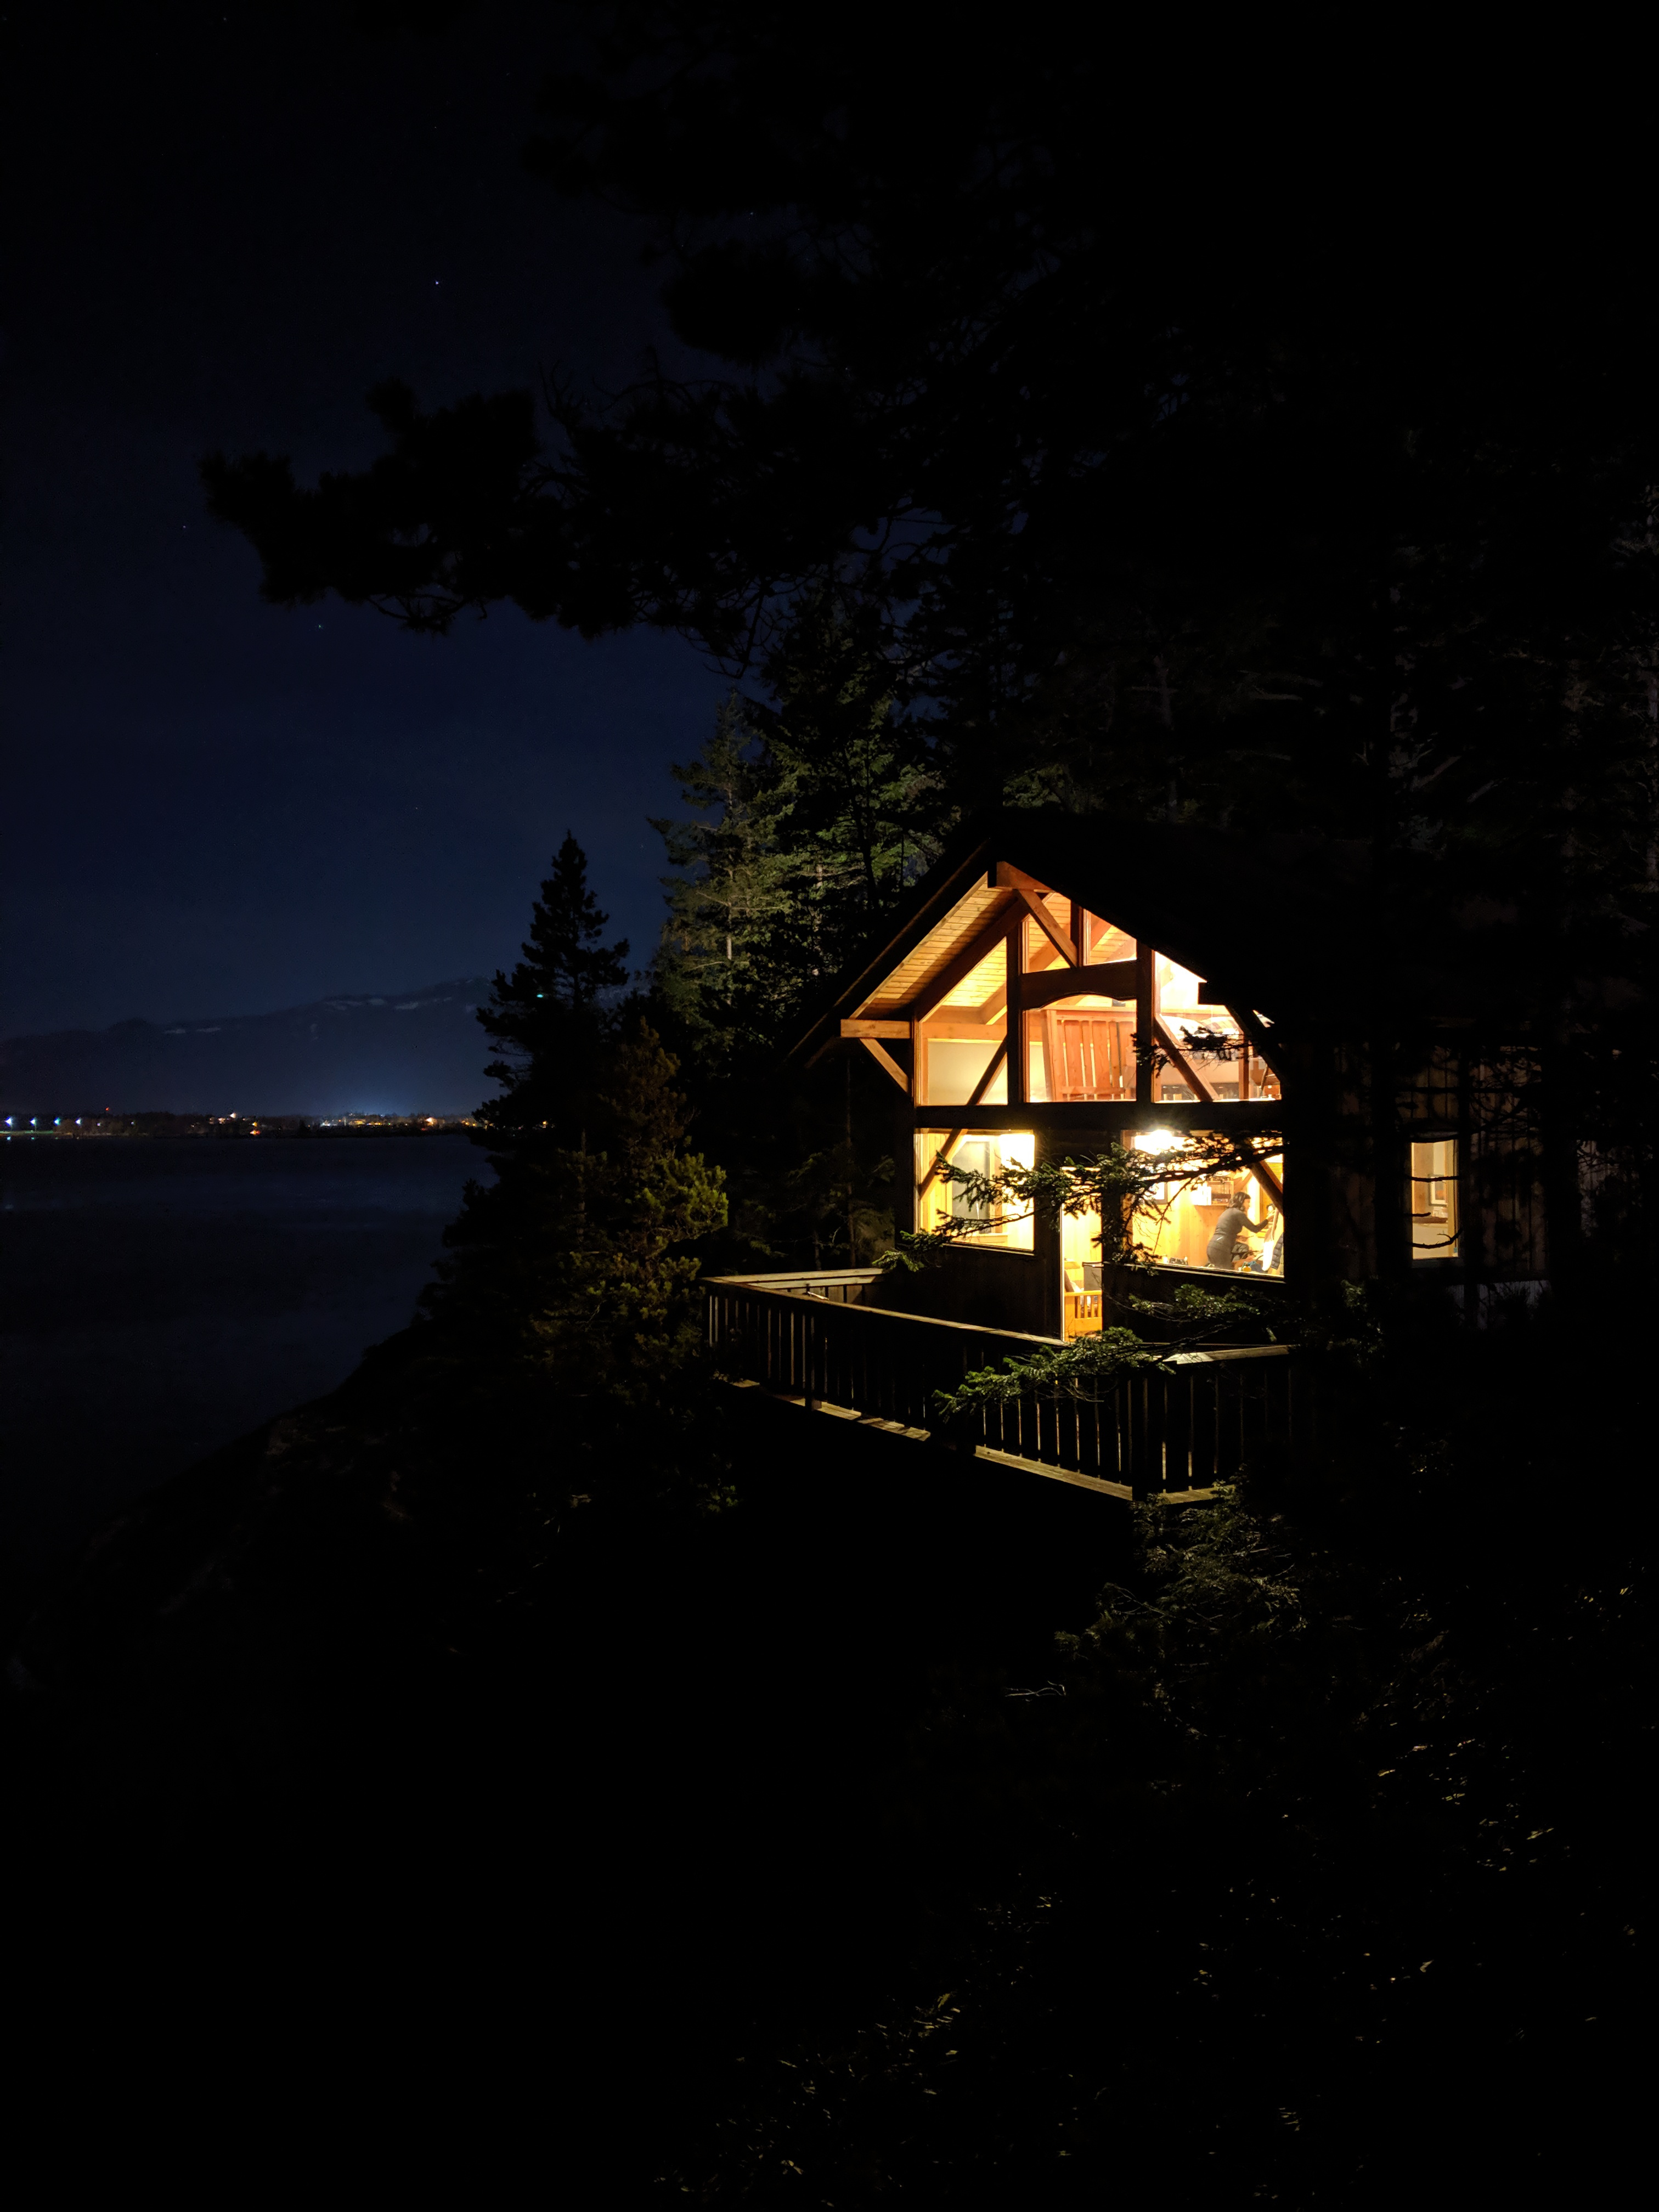
\includegraphics[width=6.5pc]{figures/liba2019-figure-14a-95quality.jpg}
\caption{Baseline}
\label{fig:toneMapping:baseline}
\end{subfigure}
\begin{subfigure}{6.5pc}
\centering
\includegraphics[width=6.5pc]{figures/liba2019-figure-14b-95quality.jpg}
\caption{CLAHE}
\label{fig:toneMapping:clahe}
\end{subfigure}
\begin{subfigure}{6.5pc}
\centering
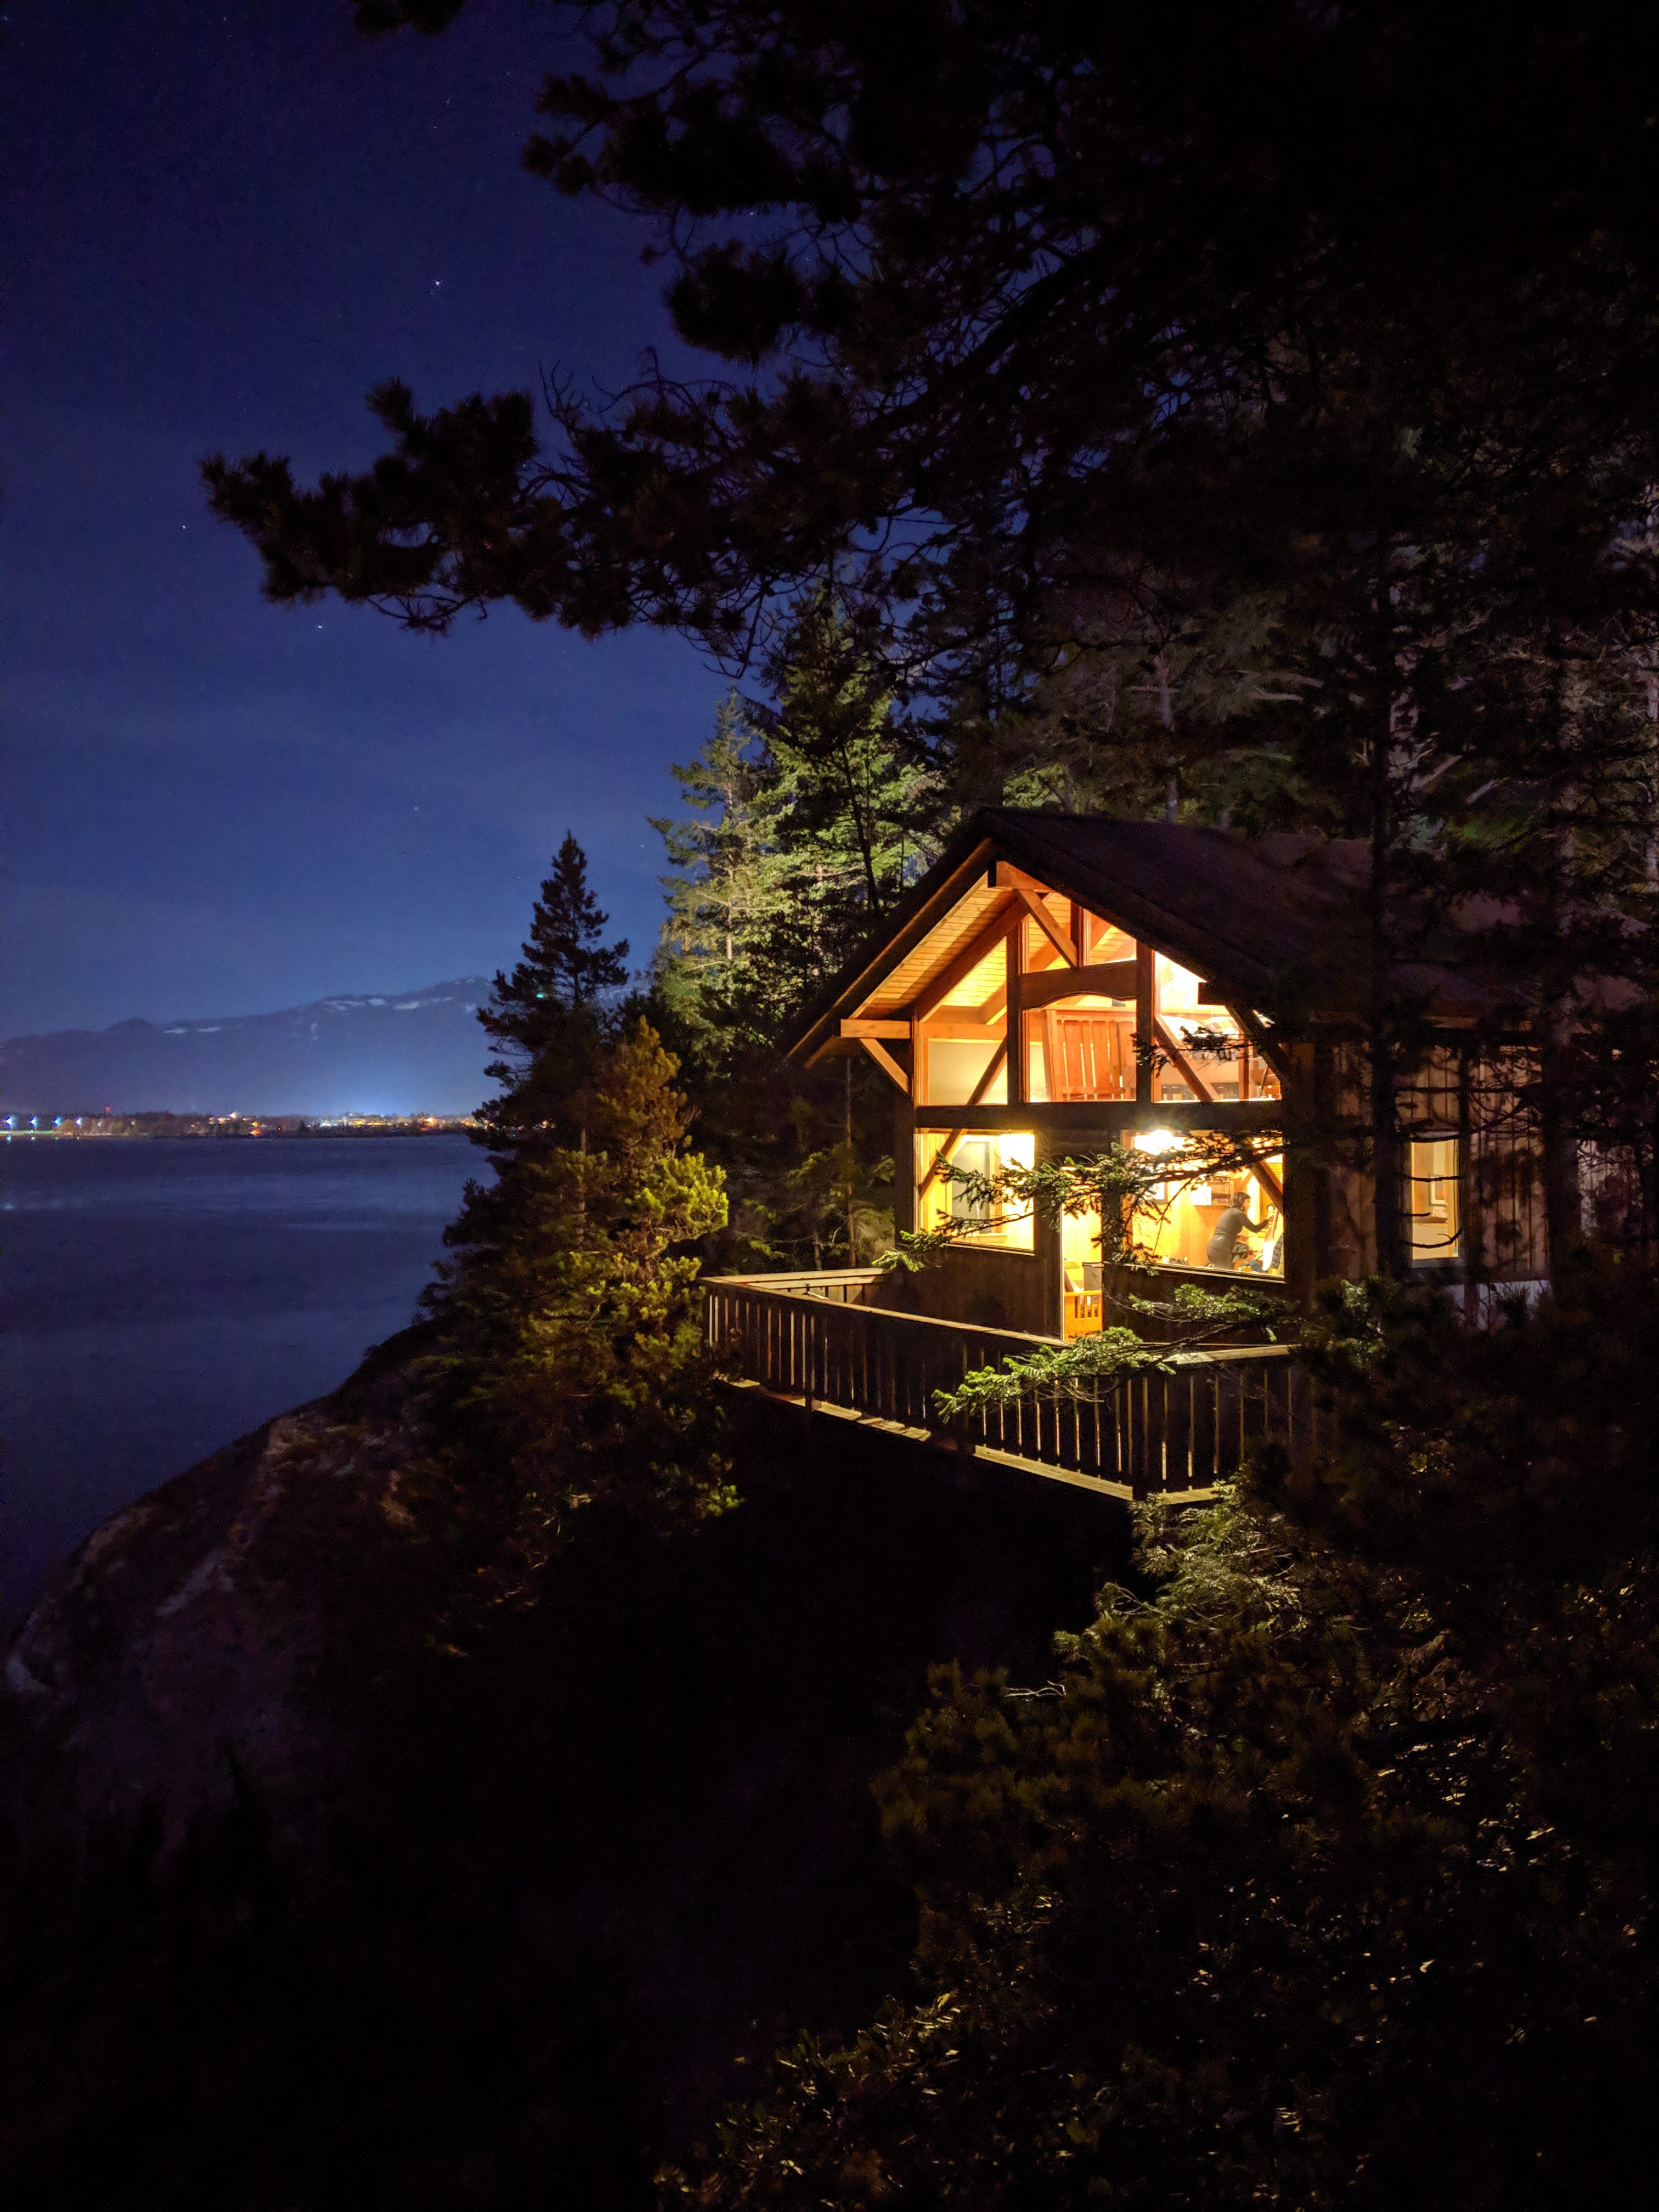
\includegraphics[width=6.5pc]{figures/liba2019-figure-14c-95quality.jpg}
\caption{Liba et al.}
\label{fig:toneMapping:liba}
\end{subfigure}

\caption{An example of tone mapping a night scene. The tone mapping of Hasinoff et al. \cite{Hasinoff2016} (\textbf{a}) produces too dark of an image while using a different tone mapping technique (\textbf{b}) that brightens using histogram equalization (CLAHE~\cite{CLAHE}) results in more detail but lacking global contrast. The tone mapping from Liba et al. (\textbf{c}) retains detail while keeping global contrast and dark areas to look like a night scene.~\cite{Liba2019}}

\label{fig:toneMapping}
\end{figure}


\begin{figure*}
\centering
\begin{subfigure}{13.8pc}
\centering
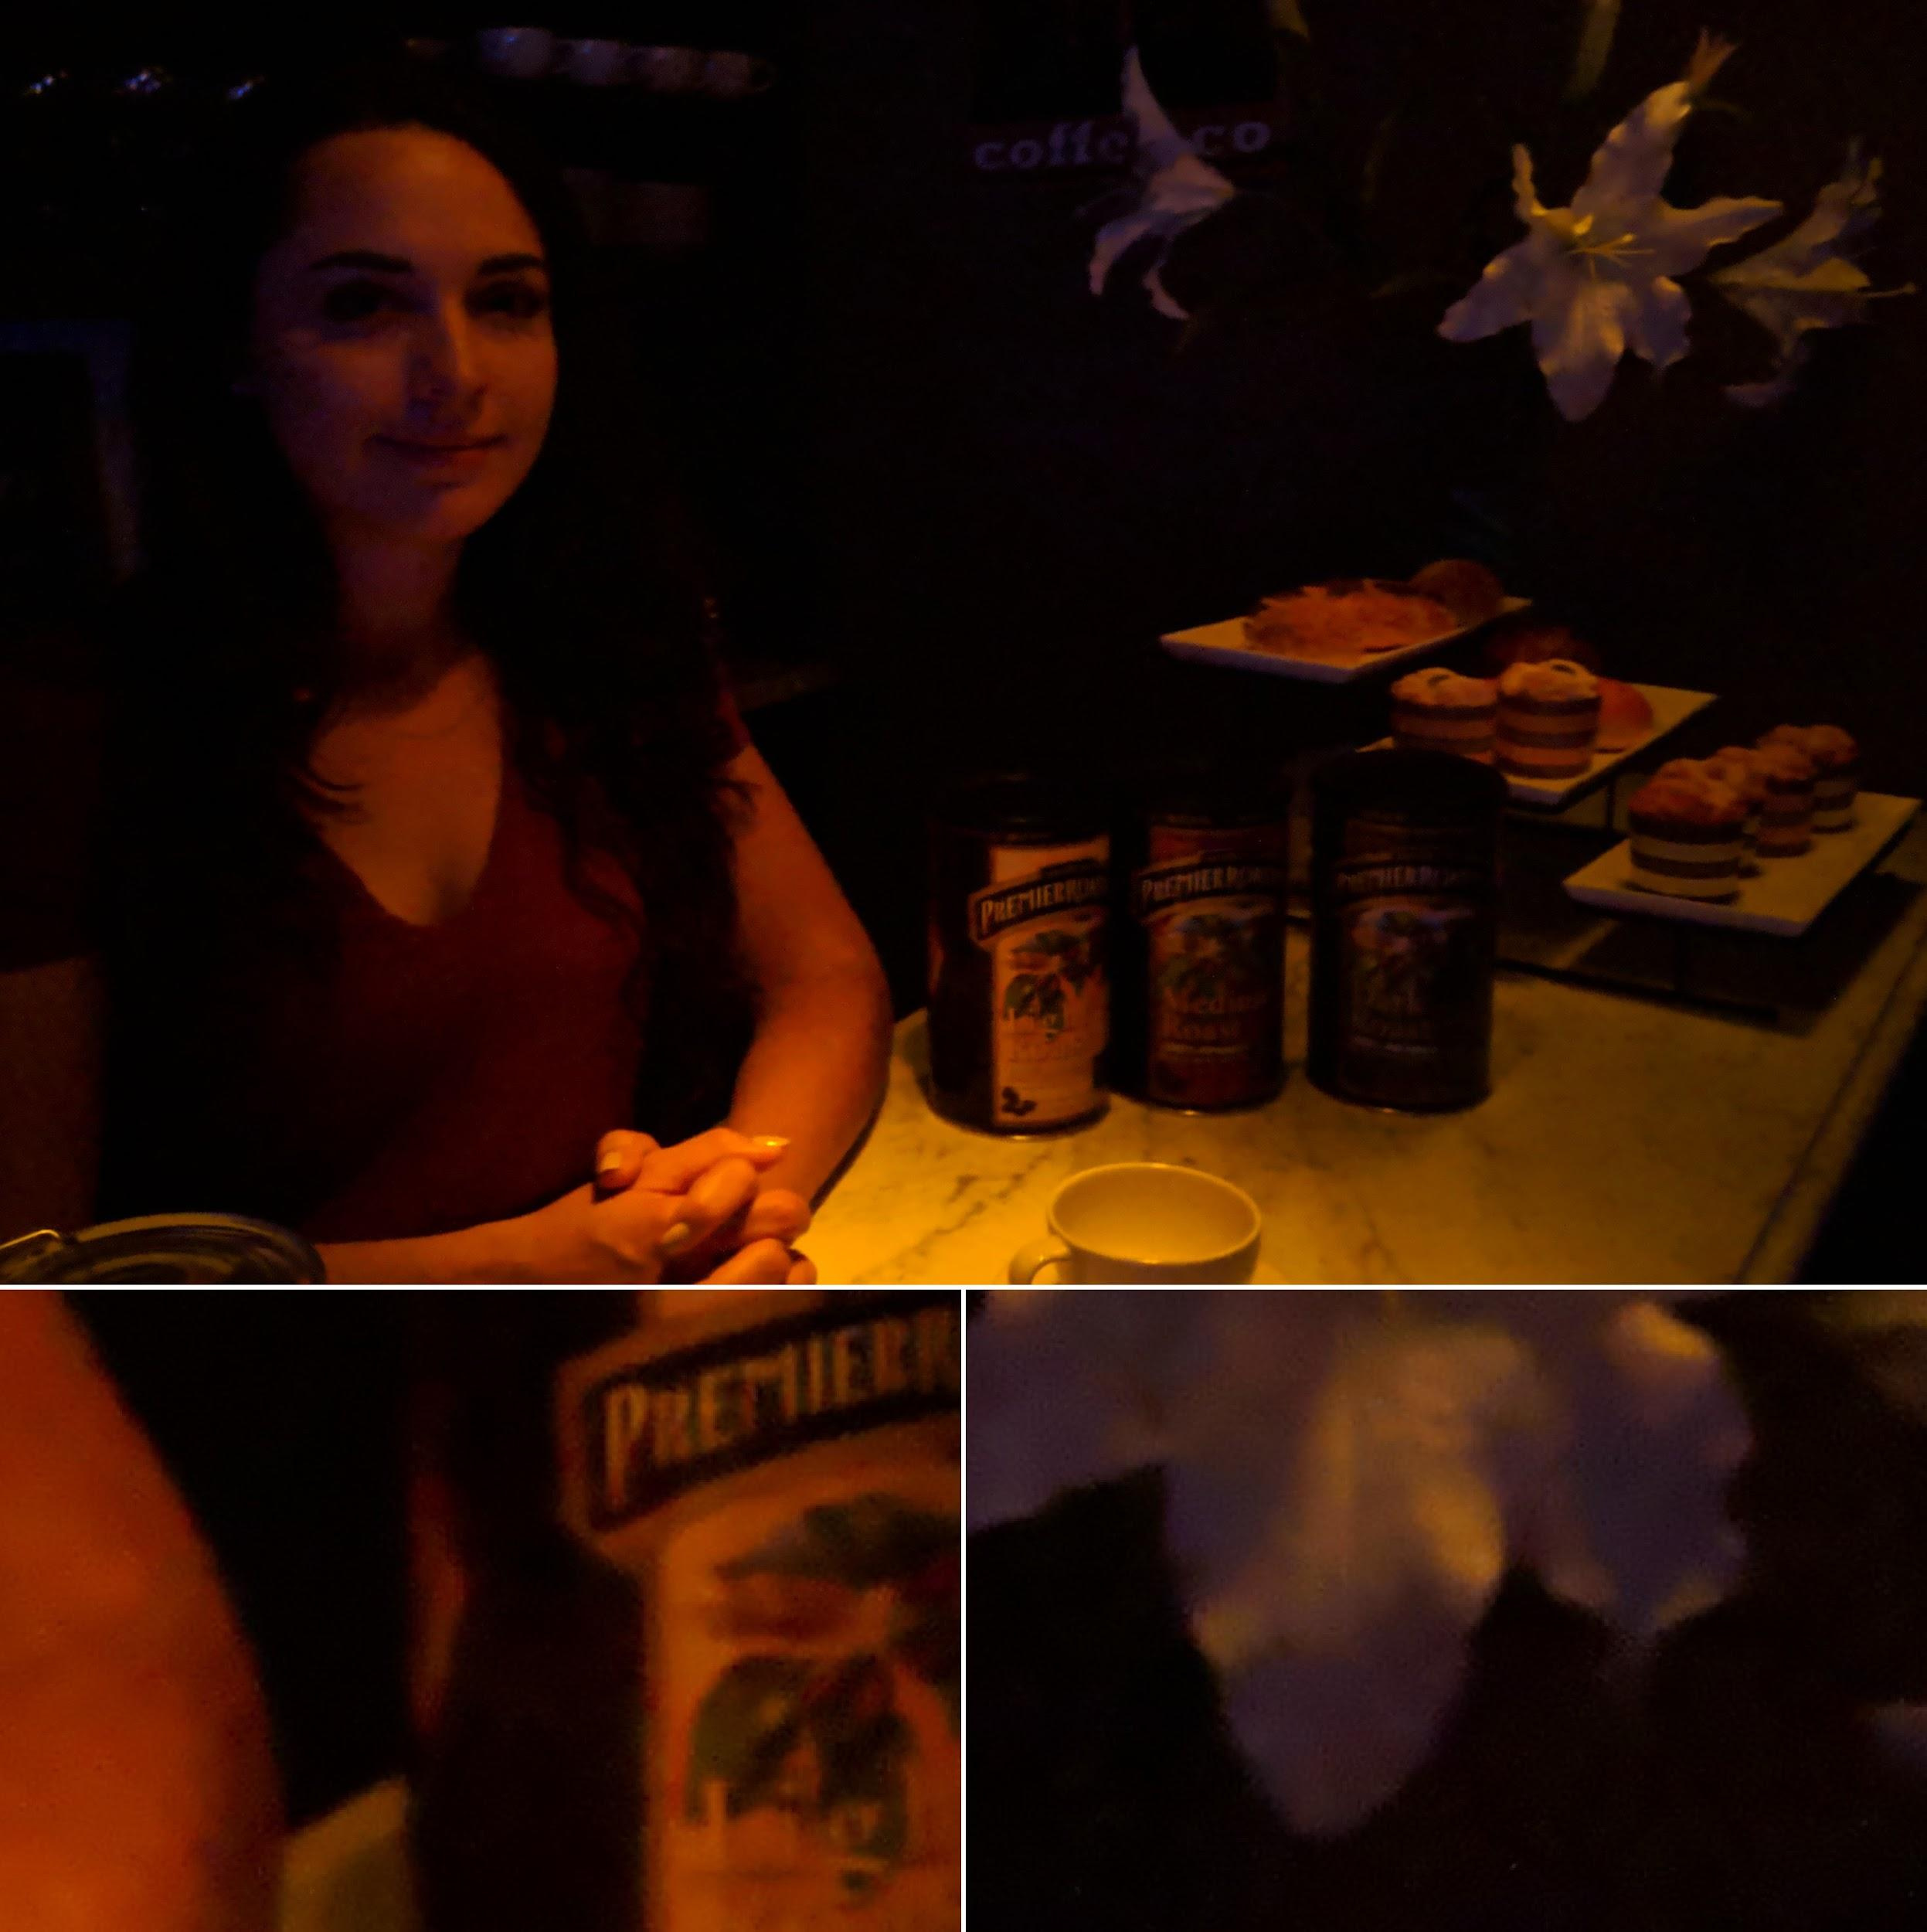
\includegraphics[width=13.8pc]{figures/liba2019-figure-1a-95quality.jpg}
\caption{Hasinoff et al.}
\label{fig:libaResults:hasinoff}
\end{subfigure}
\begin{subfigure}{13.8pc}
\centering
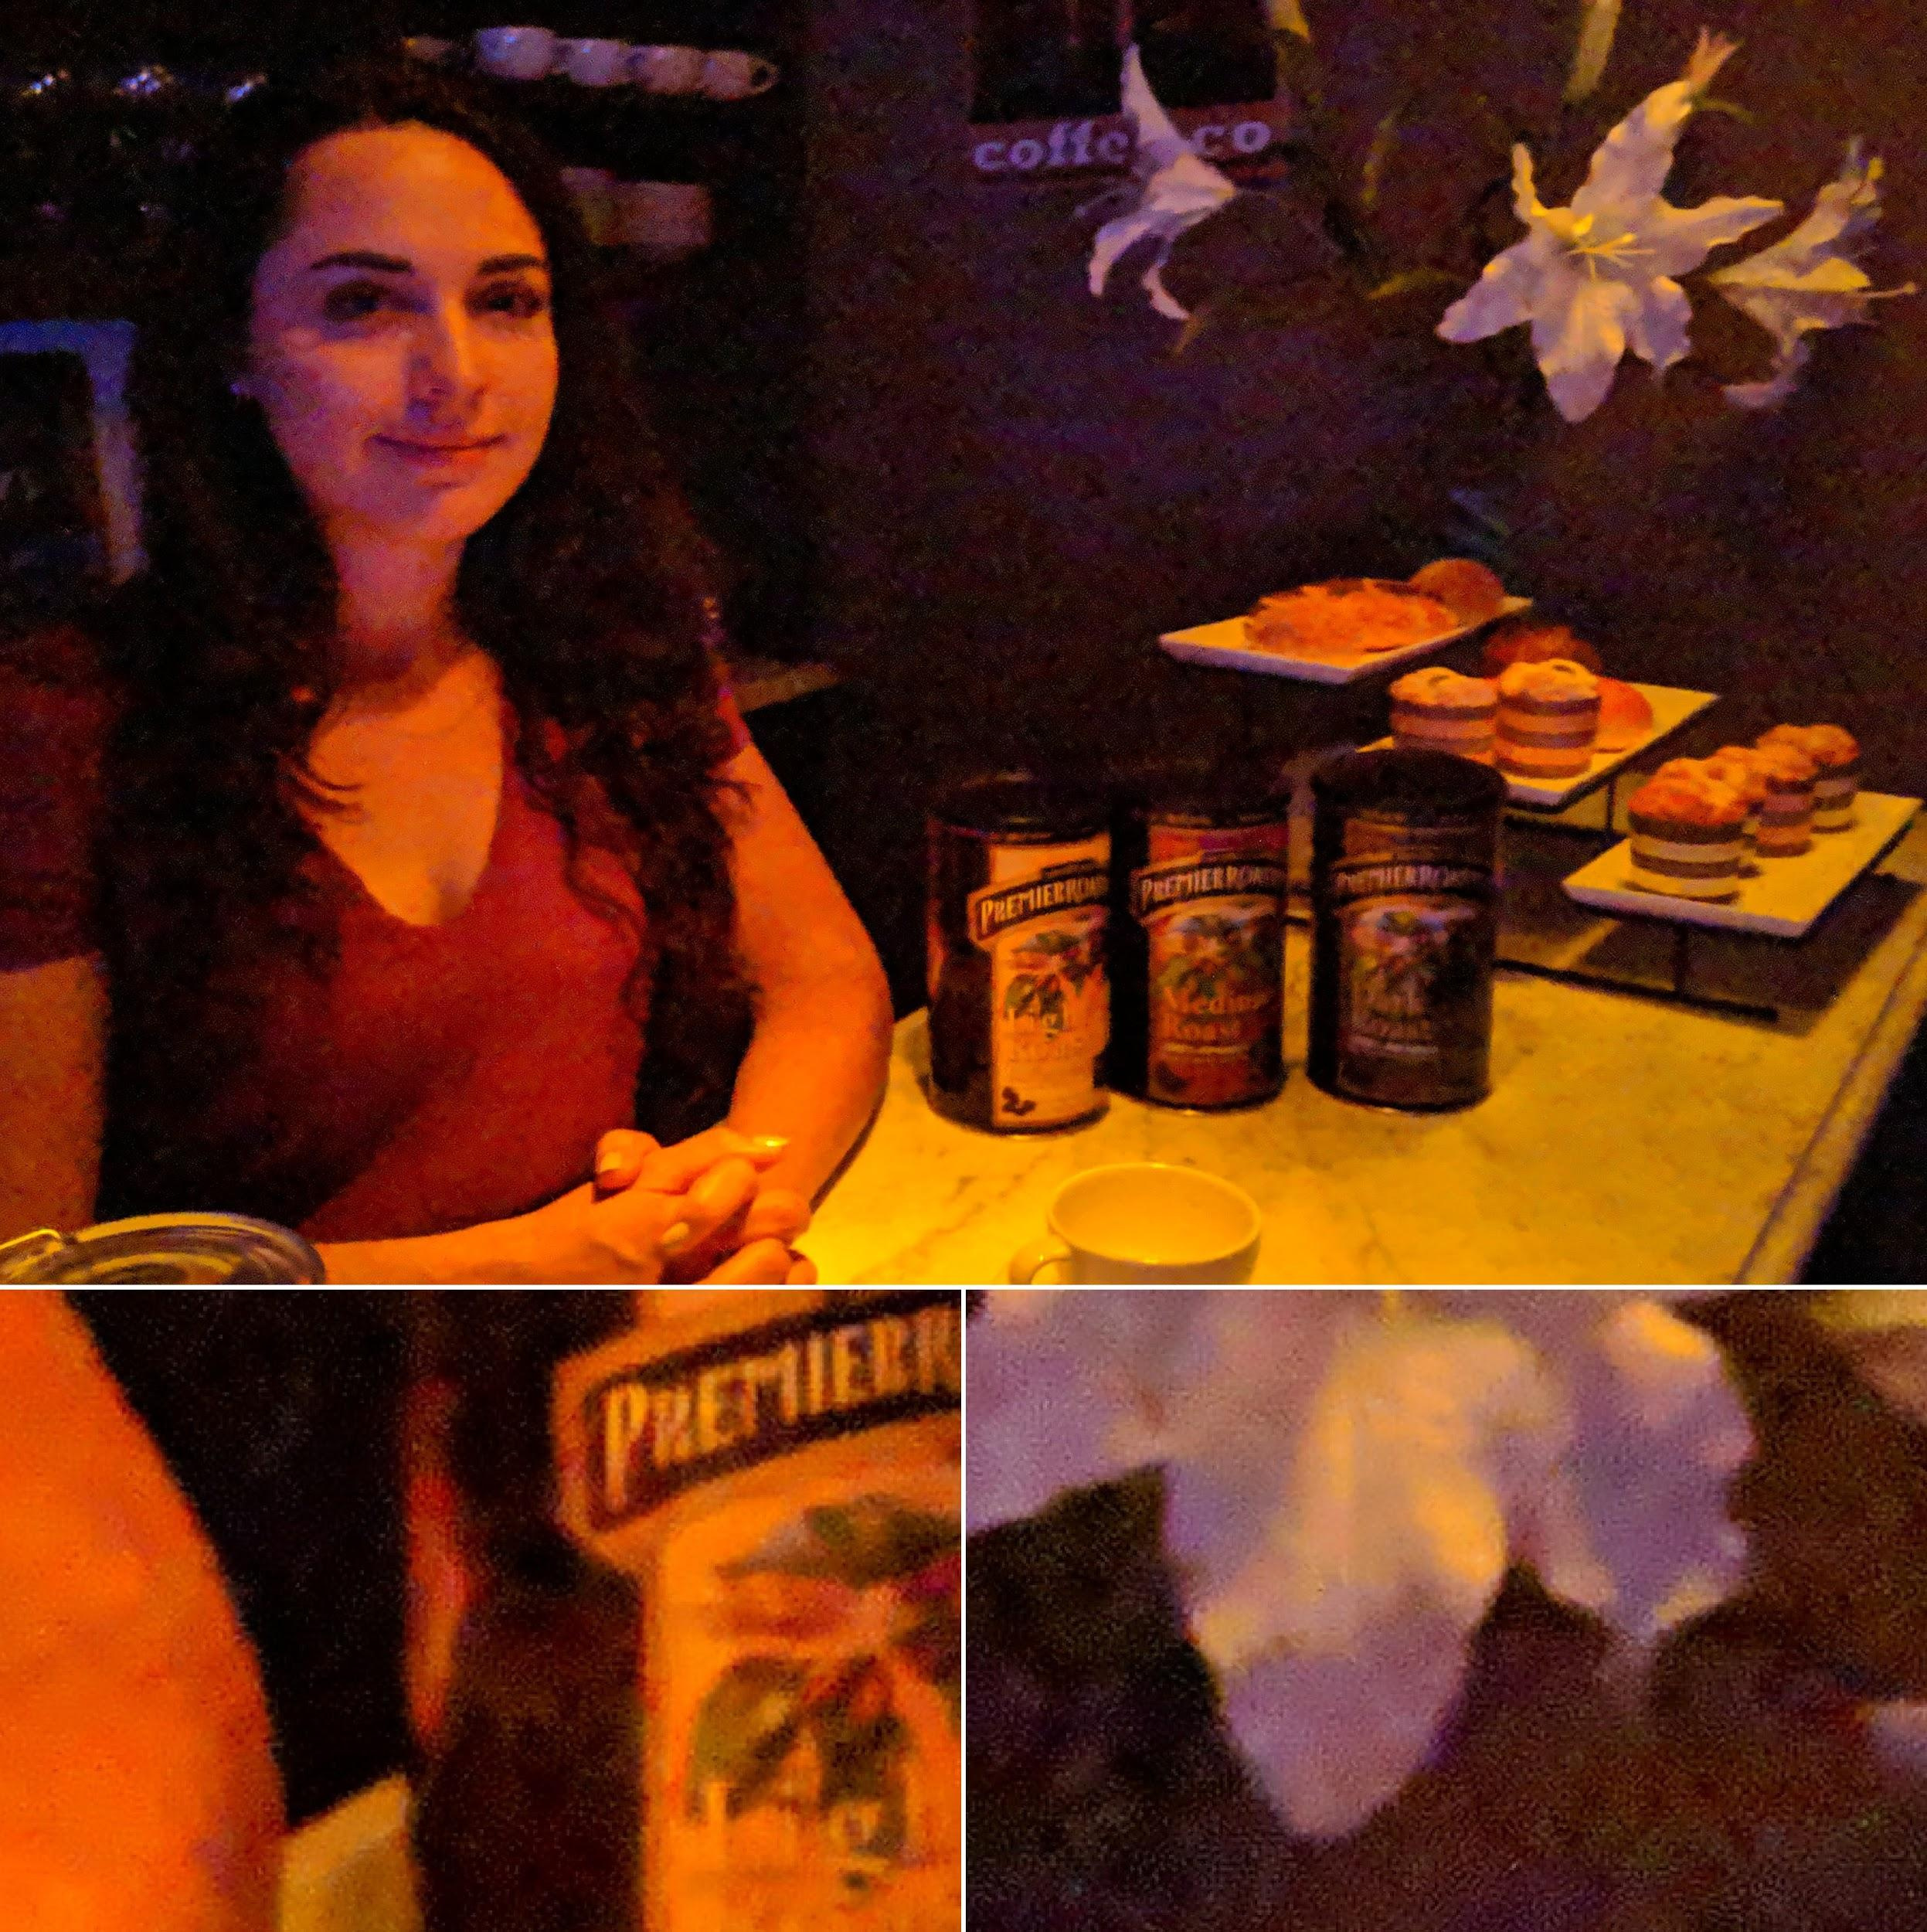
\includegraphics[width=13.8pc]{figures/liba2019-figure-1b-95quality.jpg}
\caption{Hasinoff et al. brightened}
\label{fig:libaResults:Hasinoff}
\end{subfigure}
\begin{subfigure}{13.8pc}
\centering
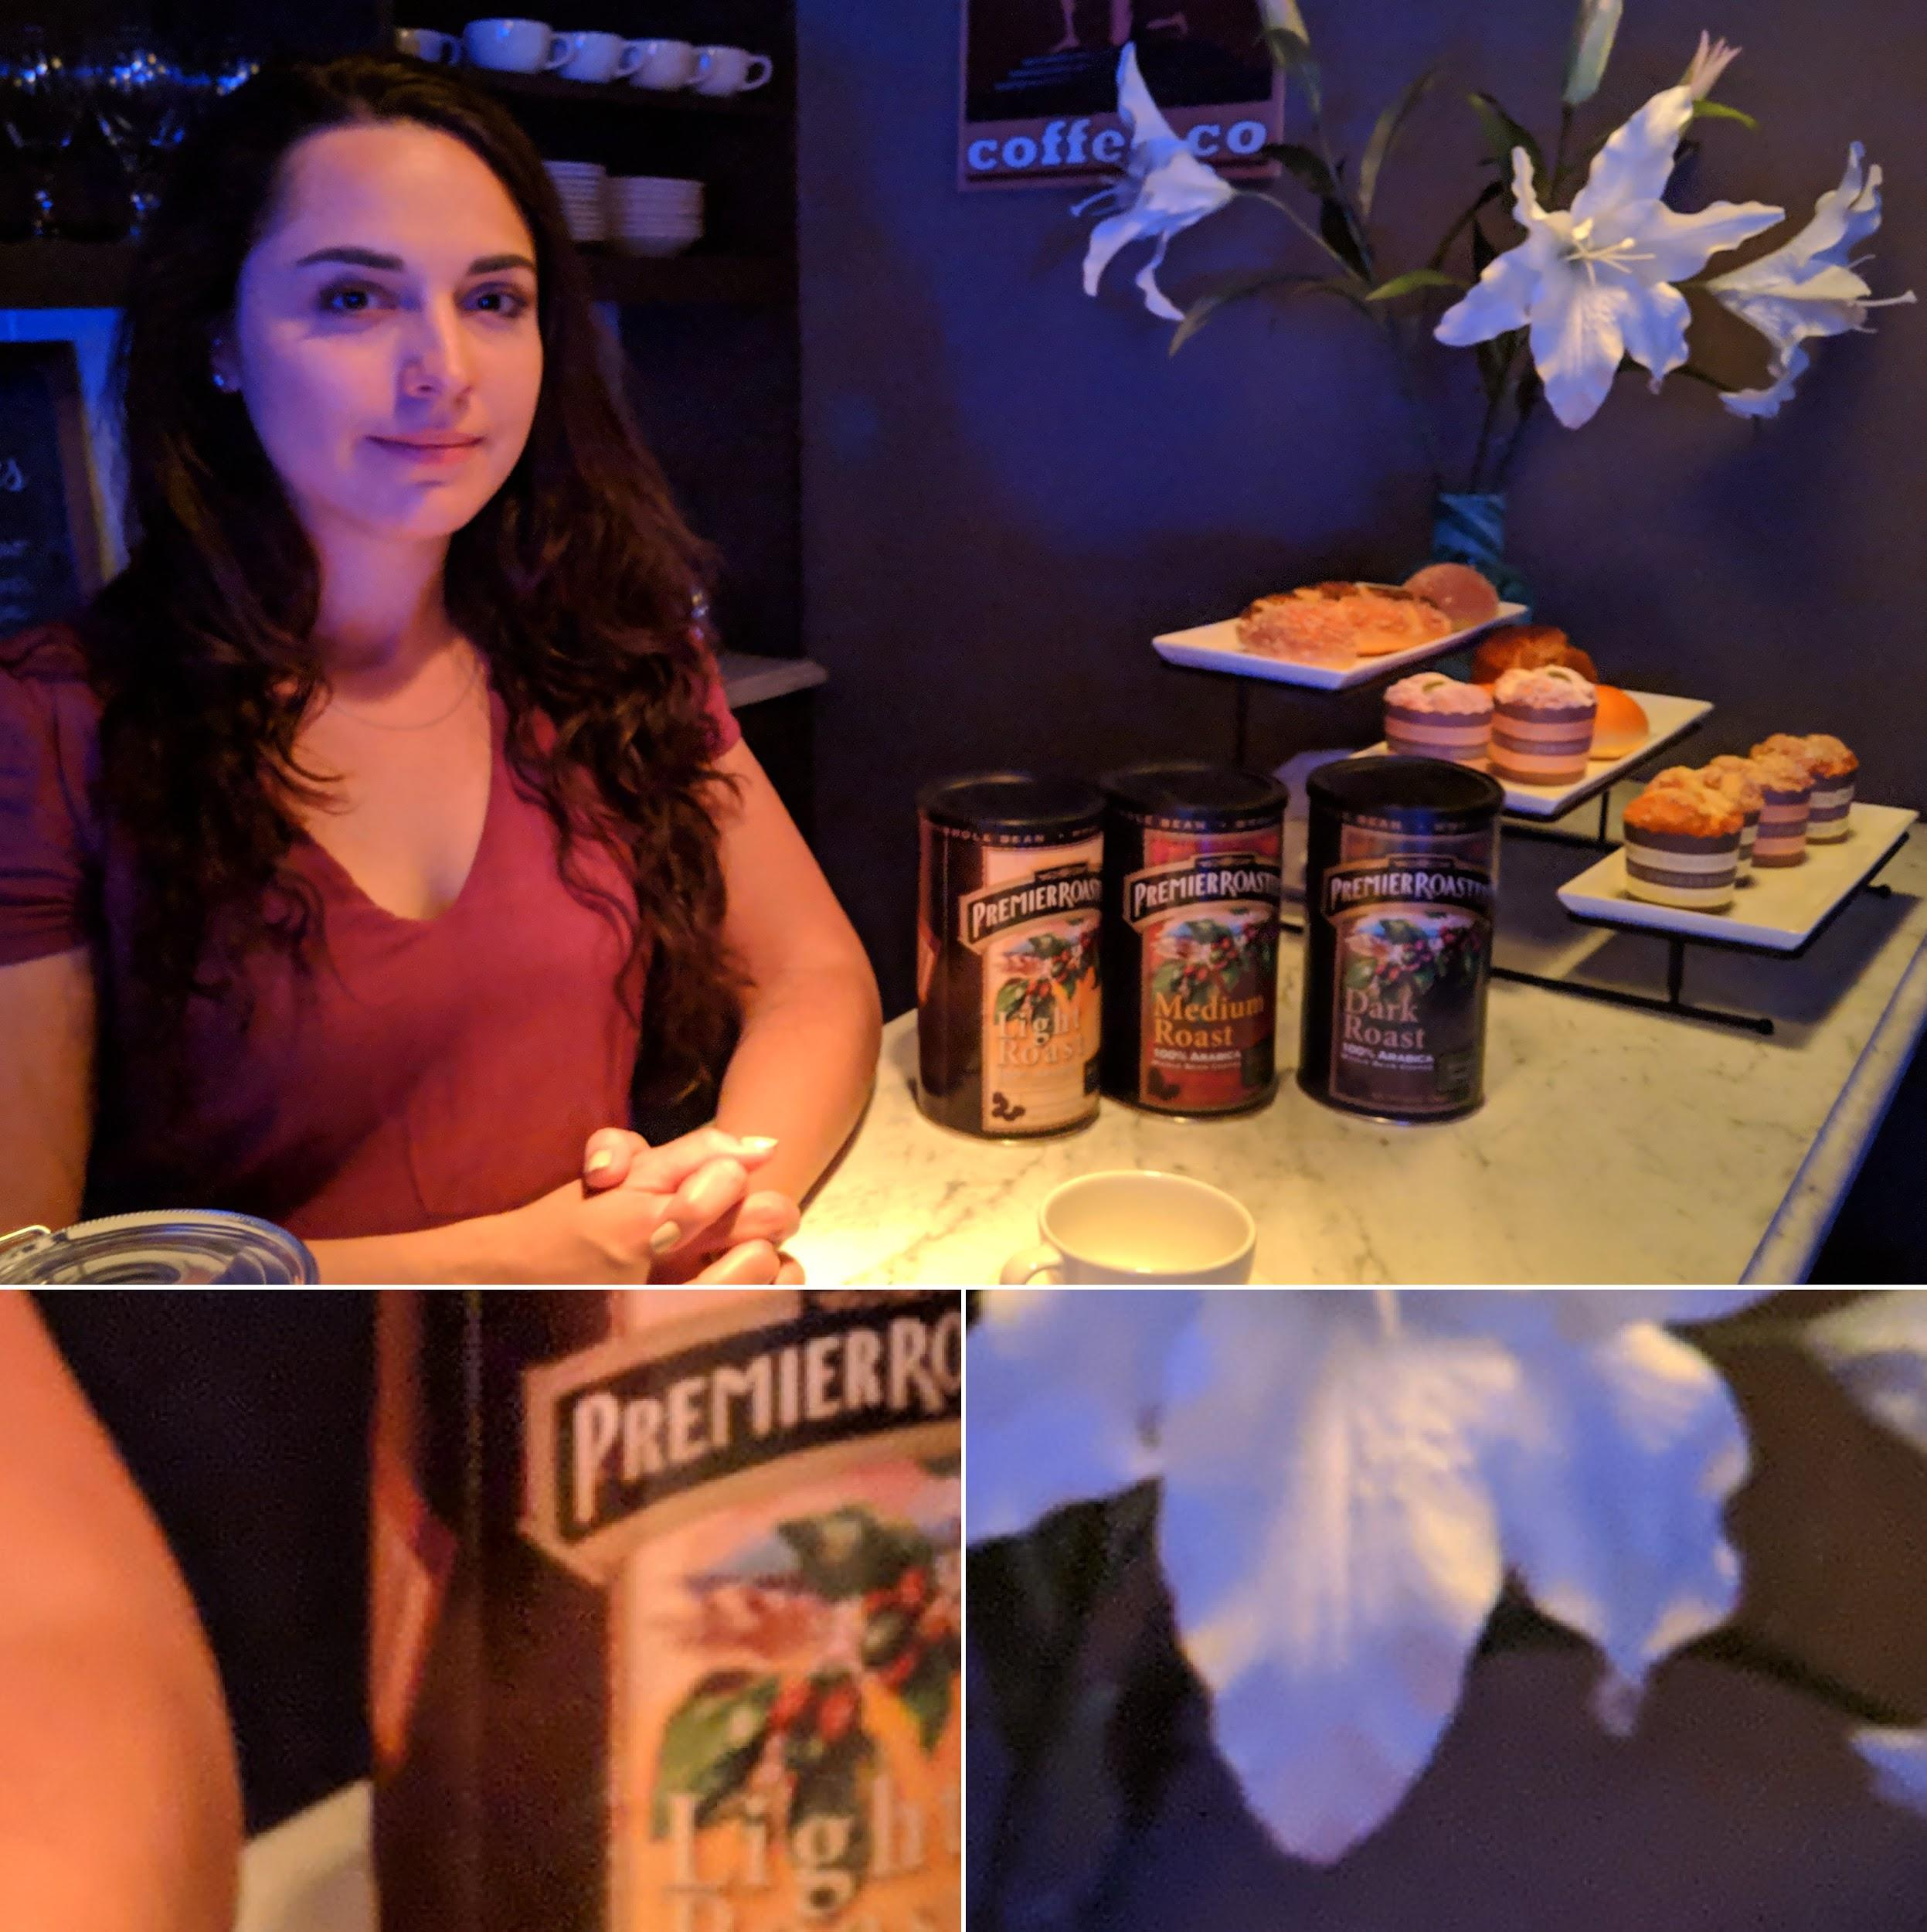
\includegraphics[width=13.8pc]{figures/liba2019-figure-1c-95quality.jpg}
\caption{Liba et al.}
\label{fig:libaResults:liba}
\end{subfigure}

\caption{A comparison of images captured using the Hasinoff et al. pipeline (a and b) and the pipeline by Liba et al. showing the improvements in detail and noise from selecting a longer exposure time due to the low motion in the scene and taking more frames. It also shows the improvements in color reproduction from the improved white balance algorithm and tone mapping.~\cite{Liba2019}}


\label{fig:libaResults}
\end{figure*}



\pagebreak

\subsection{Tone Mapping}
\label{sec:toneMapping}


Tone mapping is the process of mapping colors from a high-dynamic-range image to another in a medium with a more limited dynamic range \cite{wiki:ToneMapping}. 
This is usually done by applying what are called tone mapping operators (TMOs). Some TMOs attempt to create results close to human vision, while others produce a more artistic rendition. While human vision loses color sensitivity and spatial acuity as light levels are reduced, Liba et al. still wanted to render vibrant and colorful images in low-light rather than emulating human vision.~

Simply brightening the whole image (Figure~\ref{fig:toneMapping:clahe}) can result in low contrast and undesired saturated regions that make the image look flat. For centuries, artists have evoked a nighttime aesthetic through various methods such as the use of darker pigments, suppressed shadows, and increased contrast (Figure~\ref{fig:theOrrery}).
Liba et al. developed a TMO, inspired by artistic techniques, that maintains vibrant color in dark scenes without looking artificial while still maintaining a nighttime aesthetic.

Their TMO uses various heuristics on top of the tone mapping of Hasinoff et al.~\cite{Hasinoff2016}. These include allowing higher overall gains, limiting the boosting of shadows, allowing compression of higher dynamic ranges, boosting the color saturation inversely to scene brightness, and adding a vignette (darkening around the edges of the image).
It produces a more detailed image while maintaining global contrast and the nighttime aesthetic (Figure~\ref{fig:toneMapping:liba}).

\subsection{Results}



This system by Liba et al. was launched in November 2018 on Pixel phones as the ``Night Sight" mode in the camera app. On Pixel, Pixel 2, and Pixel 3a it uses a burst merging technique adapted from Hasinoff et al. \cite{Hasinoff2016} to better handle motion while on faster Pixel phones it uses the super-resolution merging algorithm described by Wronski et al. \cite{Wronski2019} (Section~\ref{sec:handheldSuperRes}). The comparisons and results here all use the former merging technique.

\pagebreak

Liba et al. compared their system to the pipeline it built upon from Hasinoff et al. \cite{Hasinoff2016}. Figure~\ref{fig:libaResults} shows an example of their system producing lower noise, more detail, and more pleasing colors. They also compared their pipeline with a neural network that operates on single raw images by Chen et al.~\cite{Chen2018} using frames from a similar camera to the one the neural network was trained on rather than a smartphone camera and still the system by Liba et al. produced higher-quality images and processed images much faster and using less memory.

More recently, an astrophotography mode has been added to Night Sight allowing for even longer exposures (as long as 1-4 minutes) which allows for sharp and clear images of stars and extremely dark landscapes~\cite{blog:Kainz2019}.



% ----------------------------------------
\section{Conclusions}

Computational photography has allowed for massive advances in smartphone photography, allowing phone cameras to surpass what would be expected from their limited hardware. This has allowed many more people than ever before to take high quality photographs with ease. 
The software portion of a camera has become more influential to image quality than the physical hardware.
These new computational photography techniques have allowed Google to continue using the same camera sensor hardware over multiple generations of their Pixel phones while continuing to be highly rated in photo quality. It has also enabled updates that continually improve the camera performance of previous Pixel phones to the point where they compete with the latest from other manufacturers. 
Computational photography techniques will continue to be ever more important in smartphones, professional photography, and other applications.

\section*{Acknowledgments}

I would like to thank Nic McPhee, Elena Machkasova, and Kristin Shirley for their feedback and advice.

\label{sec:acknowledgments}

\pagebreak

% The following two commands are all you need in the
% initial runs of your .tex file to
% produce the bibliography for the citations in your paper.
\bibliographystyle{abbrv}
% sample_paper.bib is the name of the BibTex file containing the
% bibliography entries. Note that you *don't* include the .bib ending here.
\bibliography{paper}  
% You must have a proper ".bib" file
%  and remember to run:
% latex bibtex latex latex
% to resolve all references

\end{document}